\documentclass["WS\space 16-17\space -\space LaTeX-Kurs\space -\space Praesentation\space -\space 2.tex"]{subfiles}

\begin{document}

\section{Tabellen}
\begin{frame}[c]
	\begin{center}
		\LARGE \textbf{Tabellen}
	\end{center}
\end{frame}
%%-----------------------------------------------------------------------------------------------%
%%------------------------------------------SUBSECTION-------------------------------------------%
%%-----------------------------------------------------------------------------------------------%
\subsection{Grundlagen}
\begin{frame}[c]
	\begin{center}
		\large Grundlagen
	\end{center}
\end{frame}
%%-----------------------------------------------------------------------------------%
%%---------------------------------------FRAME---------------------------------------%
%%-----------------------------------------------------------------------------------%
\begin{frame}[c]{Importieren des calc2latex-Makros}
	\begin{onlyenv}<1>
		\begin{figure}[htbp]
			\centering
			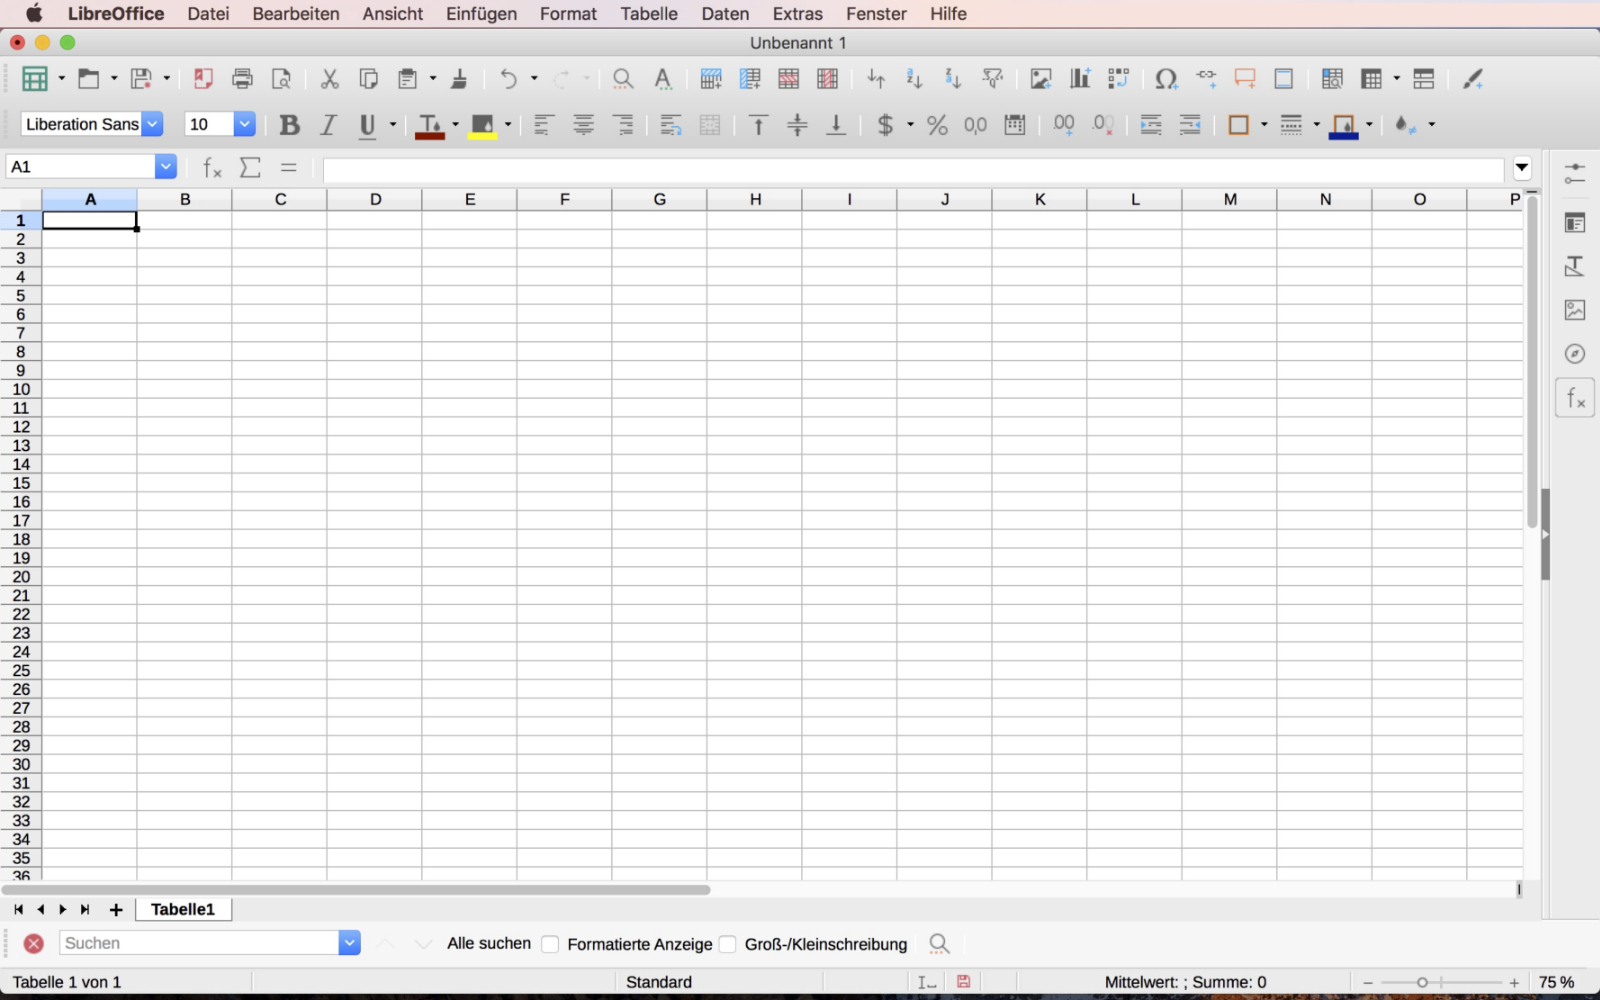
\includegraphics[width=0.9\textwidth]{img/Bildschirmfoto_mitKasten/1_Importieren_Macro/1.jpg}
		\end{figure}
	\end{onlyenv}
	\begin{onlyenv}<2>
		\begin{figure}[htbp]
			\centering
			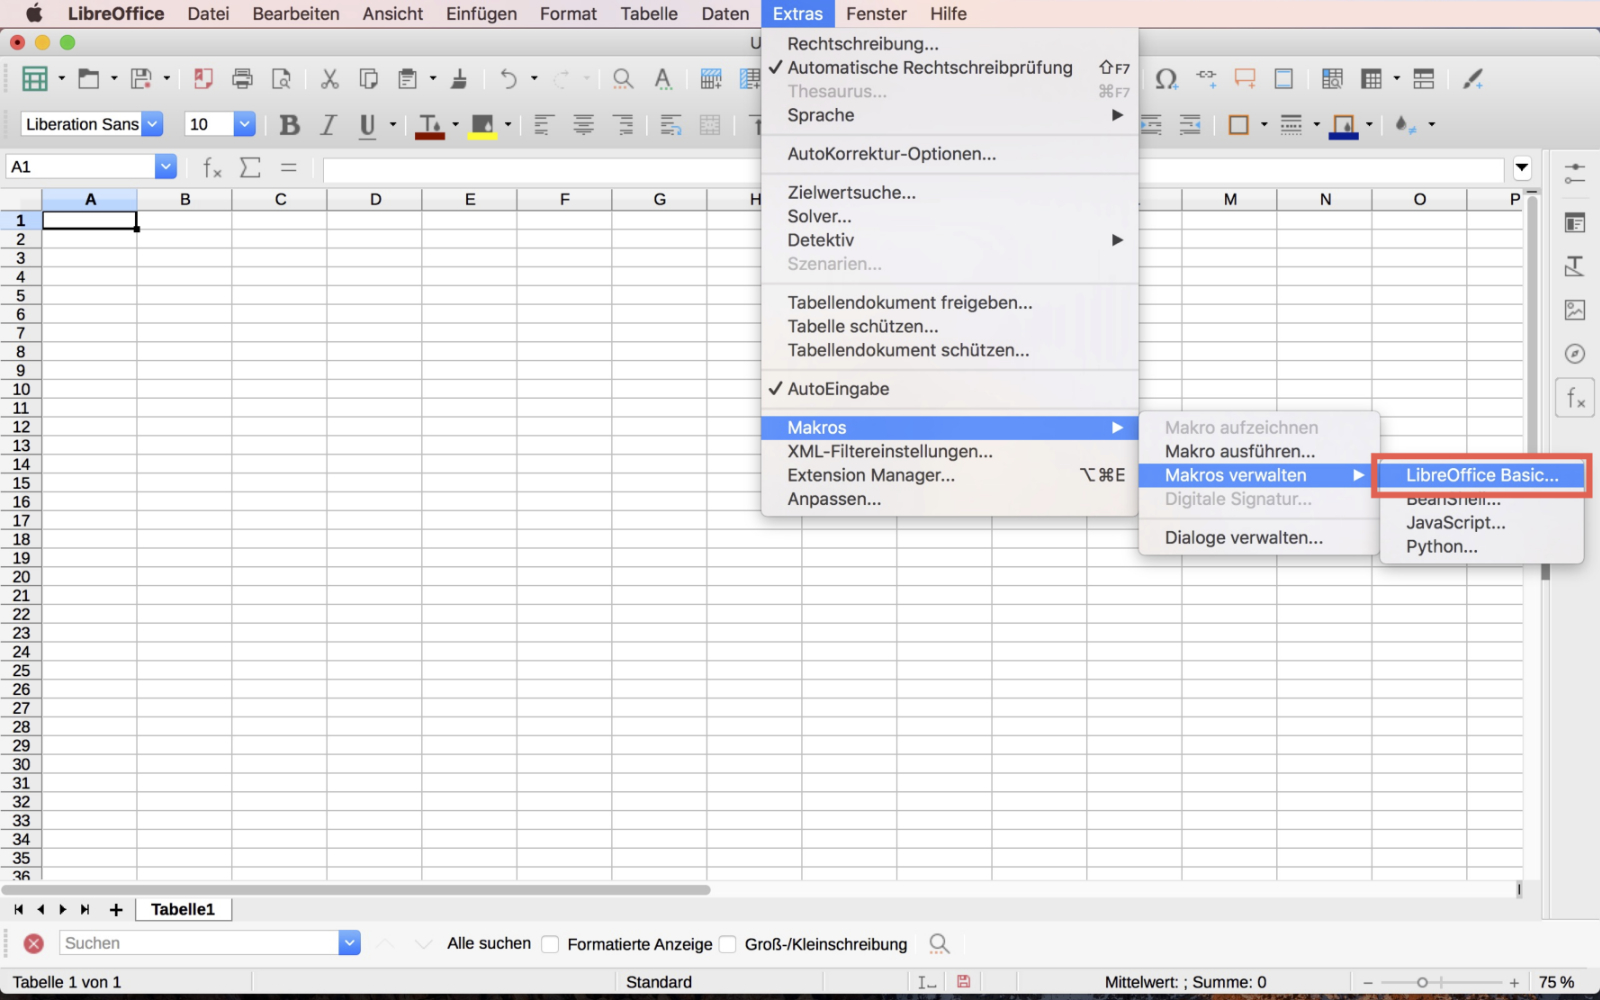
\includegraphics[width=0.9\textwidth]{img/Bildschirmfoto_mitKasten/1_Importieren_Macro/2.jpg}
		\end{figure}
	\end{onlyenv}
	\begin{onlyenv}<3>
		\begin{figure}[htbp]
			\centering
			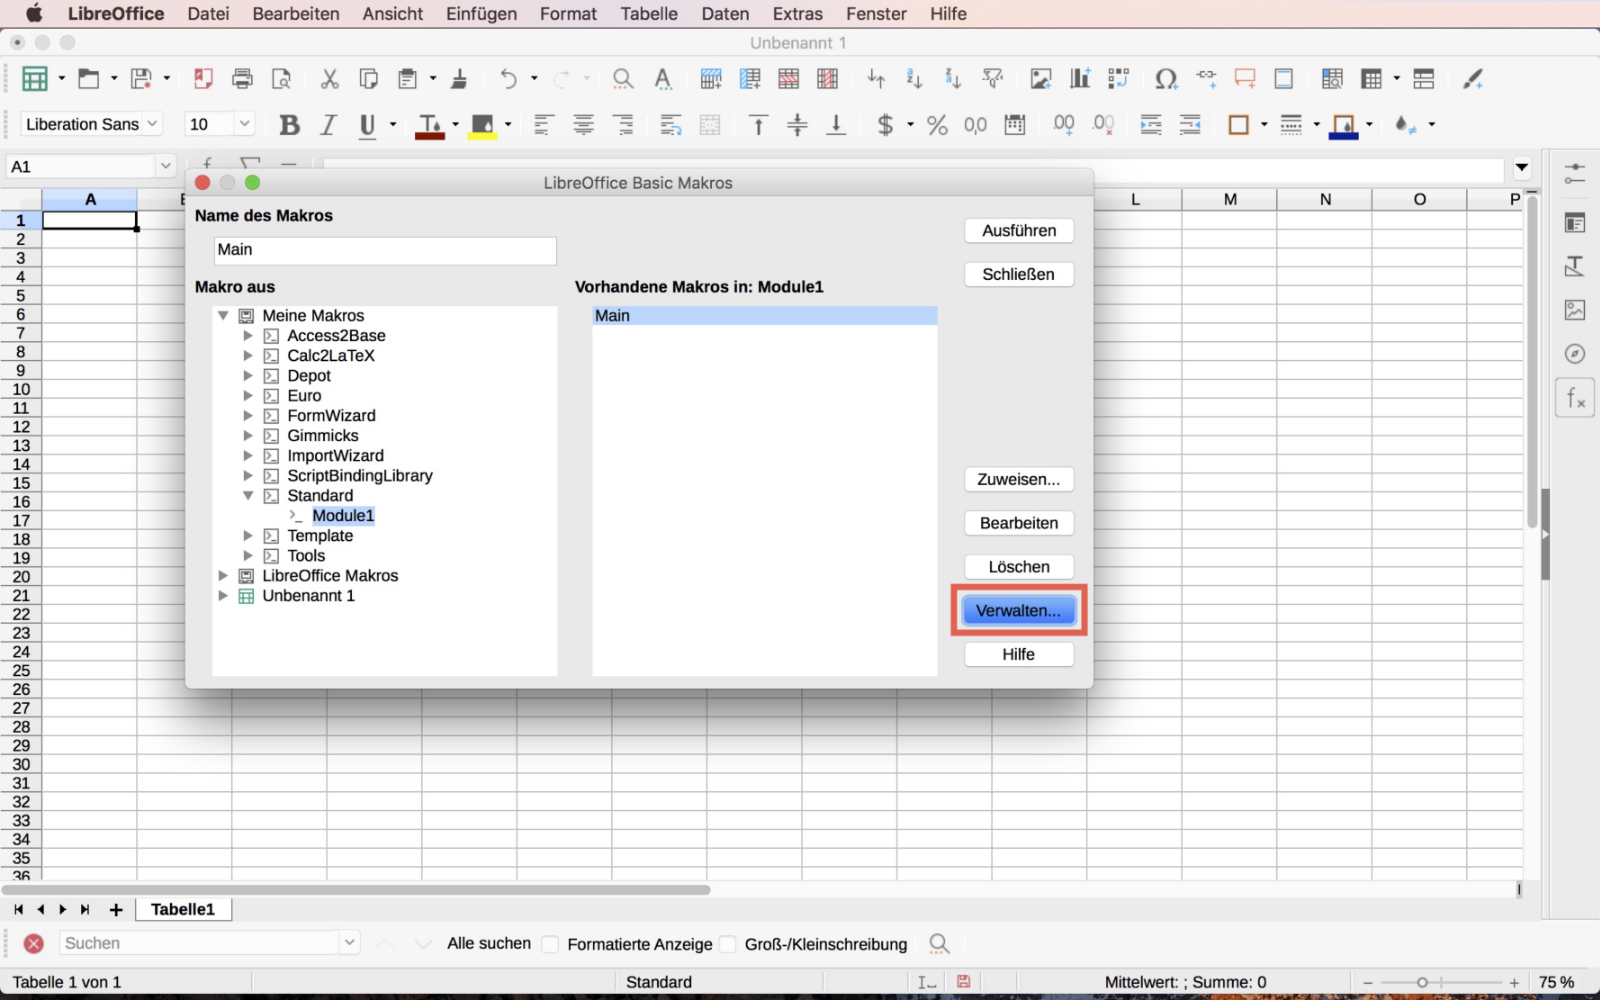
\includegraphics[width=0.9\textwidth]{img/Bildschirmfoto_mitKasten/1_Importieren_Macro/3.jpg}
		\end{figure}
	\end{onlyenv}
	\begin{onlyenv}<4>
		\begin{figure}[htbp]
			\centering
			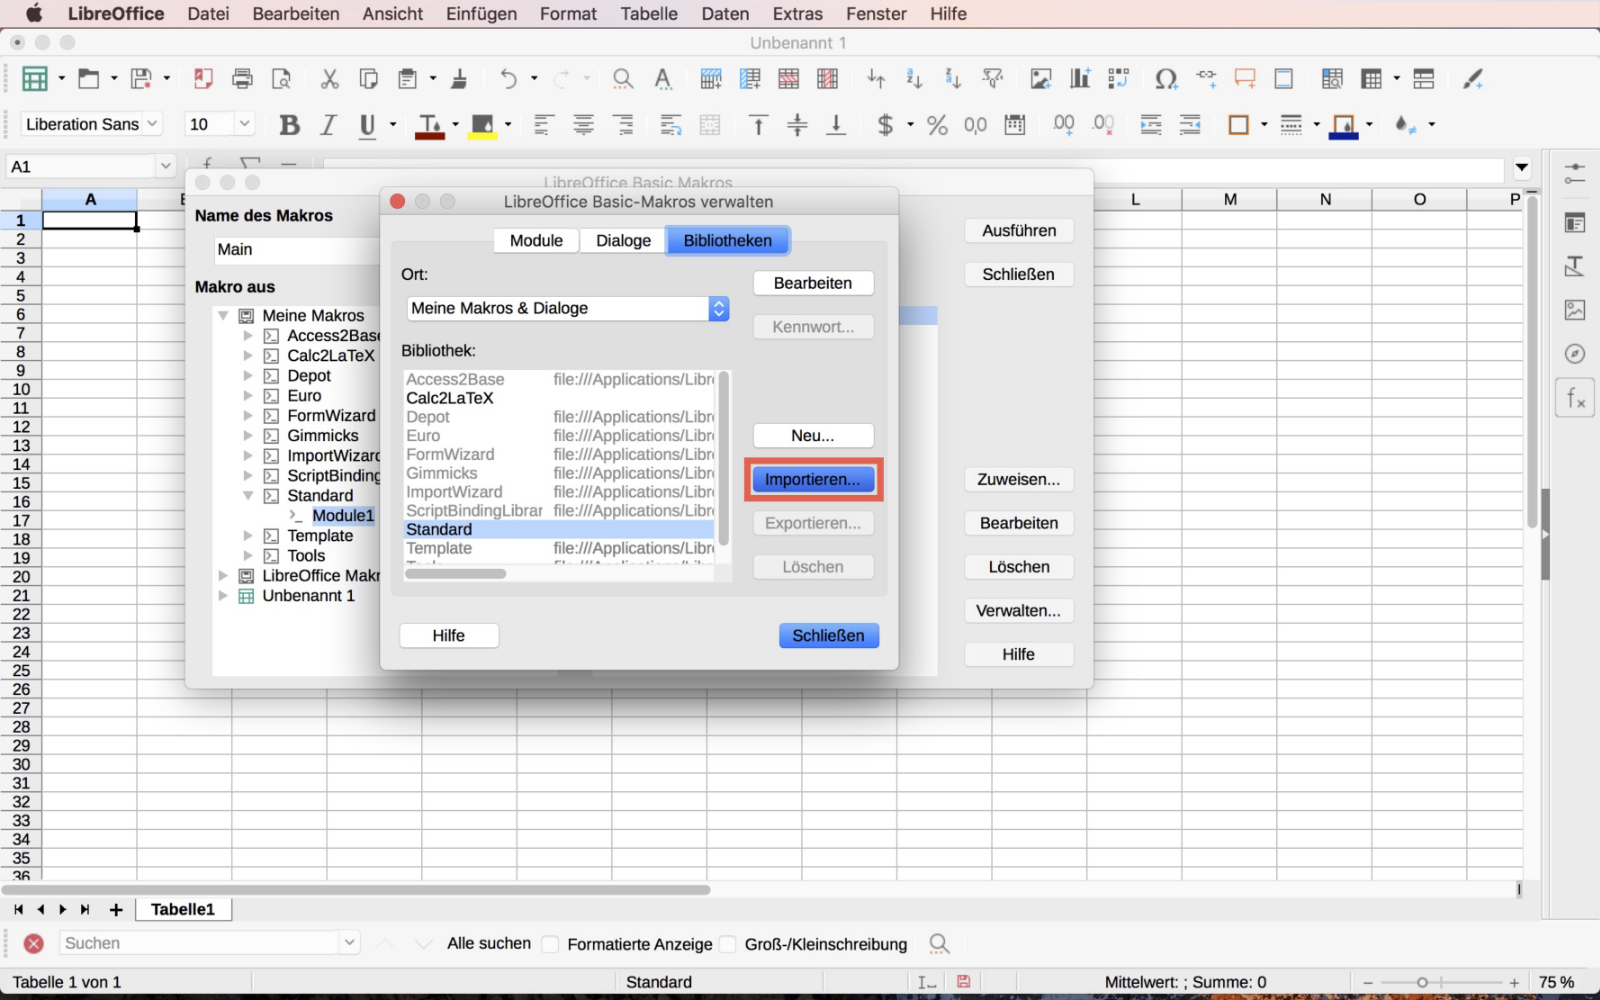
\includegraphics[width=0.9\textwidth]{img/Bildschirmfoto_mitKasten/1_Importieren_Macro/4.jpg}
		\end{figure}
	\end{onlyenv}
	\begin{onlyenv}<5>
		\begin{figure}[htbp]
			\centering
			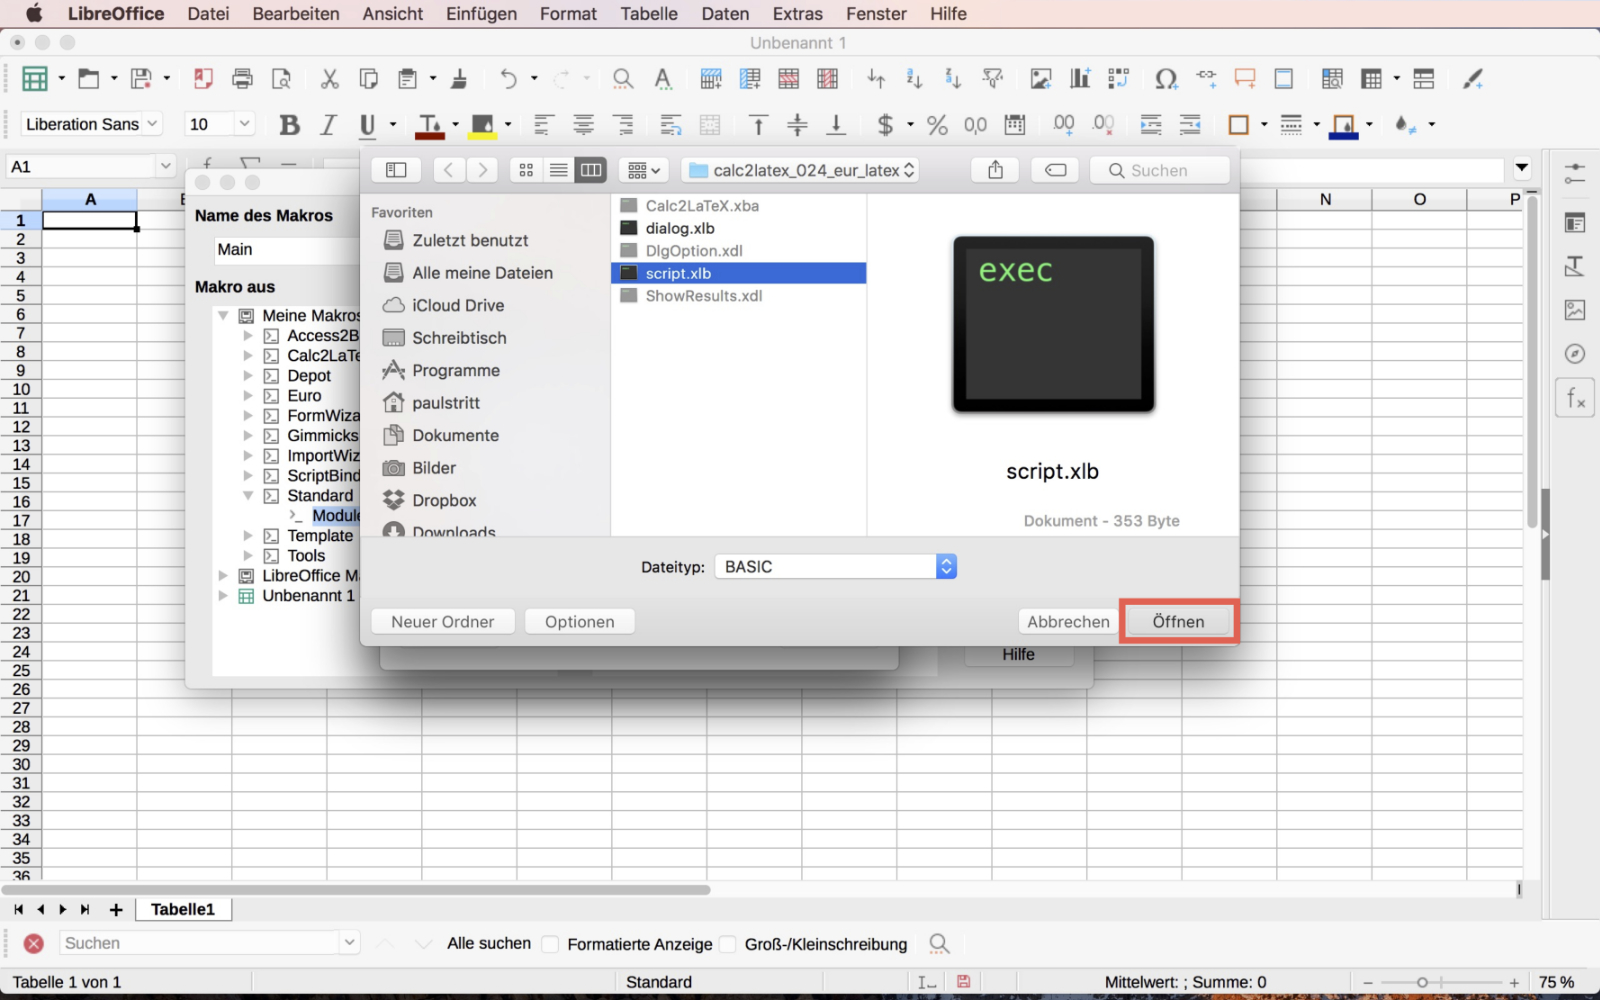
\includegraphics[width=0.9\textwidth]{img/Bildschirmfoto_mitKasten/1_Importieren_Macro/5.jpg}
		\end{figure}
	\end{onlyenv}
	\begin{onlyenv}<6>
		\begin{figure}[htbp]
			\centering
			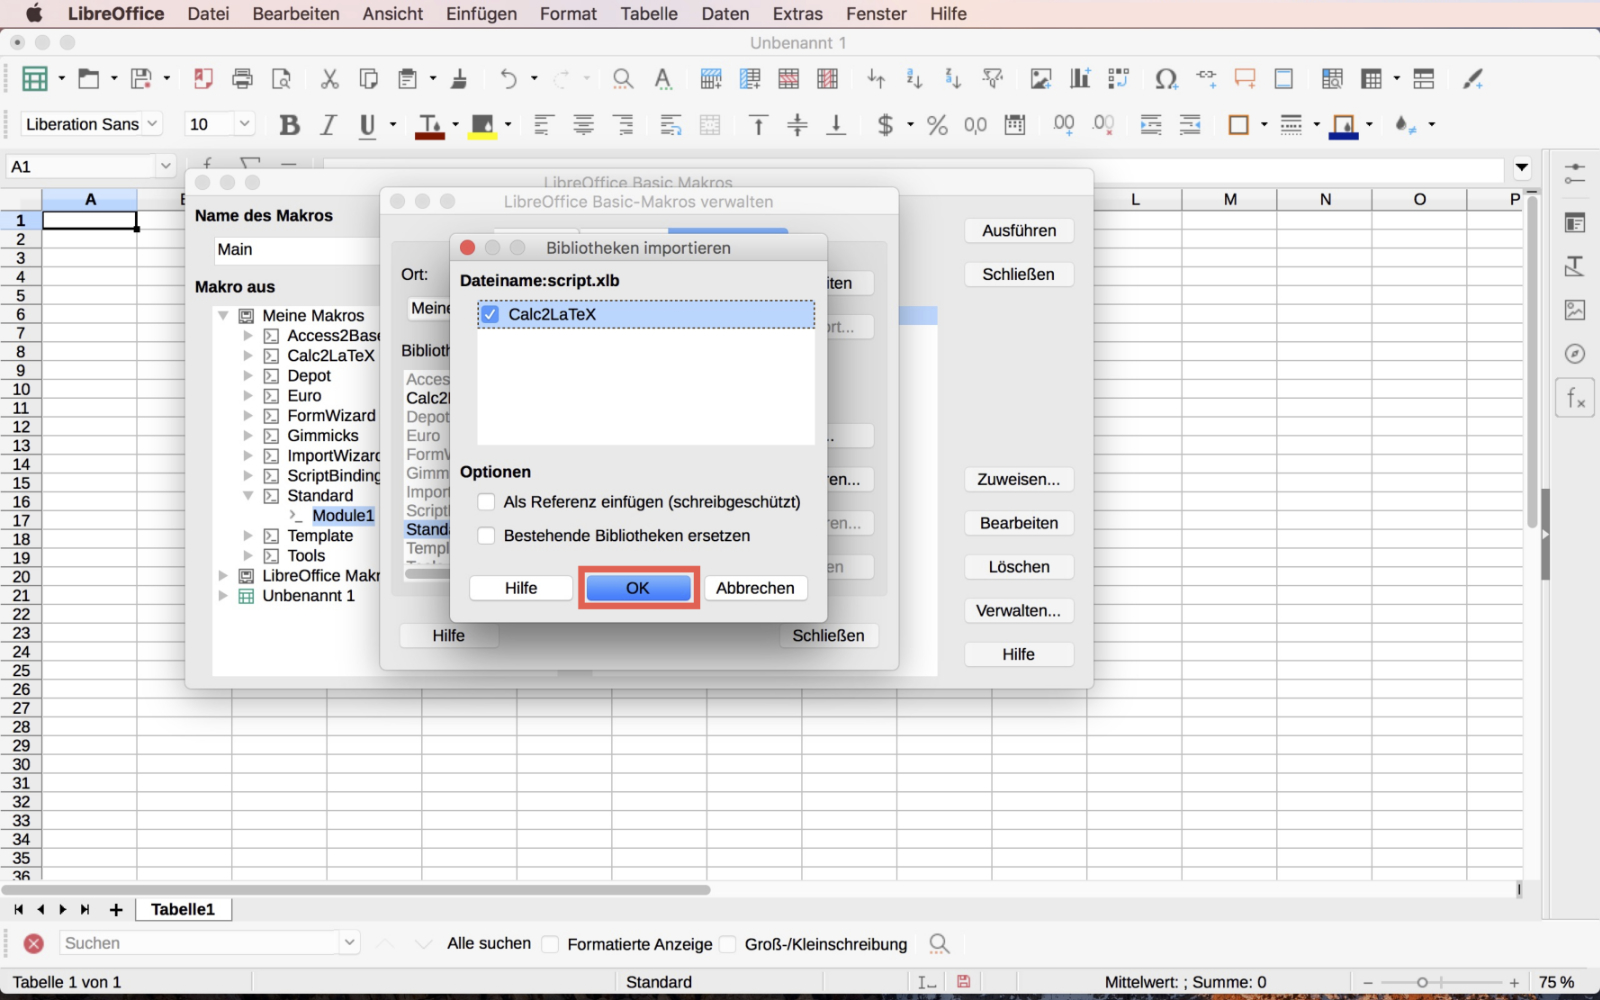
\includegraphics[width=0.9\textwidth]{img/Bildschirmfoto_mitKasten/1_Importieren_Macro/6.jpg}
		\end{figure}
	\end{onlyenv}
\end{frame}
%%-----------------------------------------------------------------------------------%
%%---------------------------------------FRAME---------------------------------------%
%%-----------------------------------------------------------------------------------%
\begin{frame}[c]{Erstellen einer Tastenkombination für calc2latex}
	\begin{onlyenv}<1>
		\begin{figure}[htbp]
			\centering
			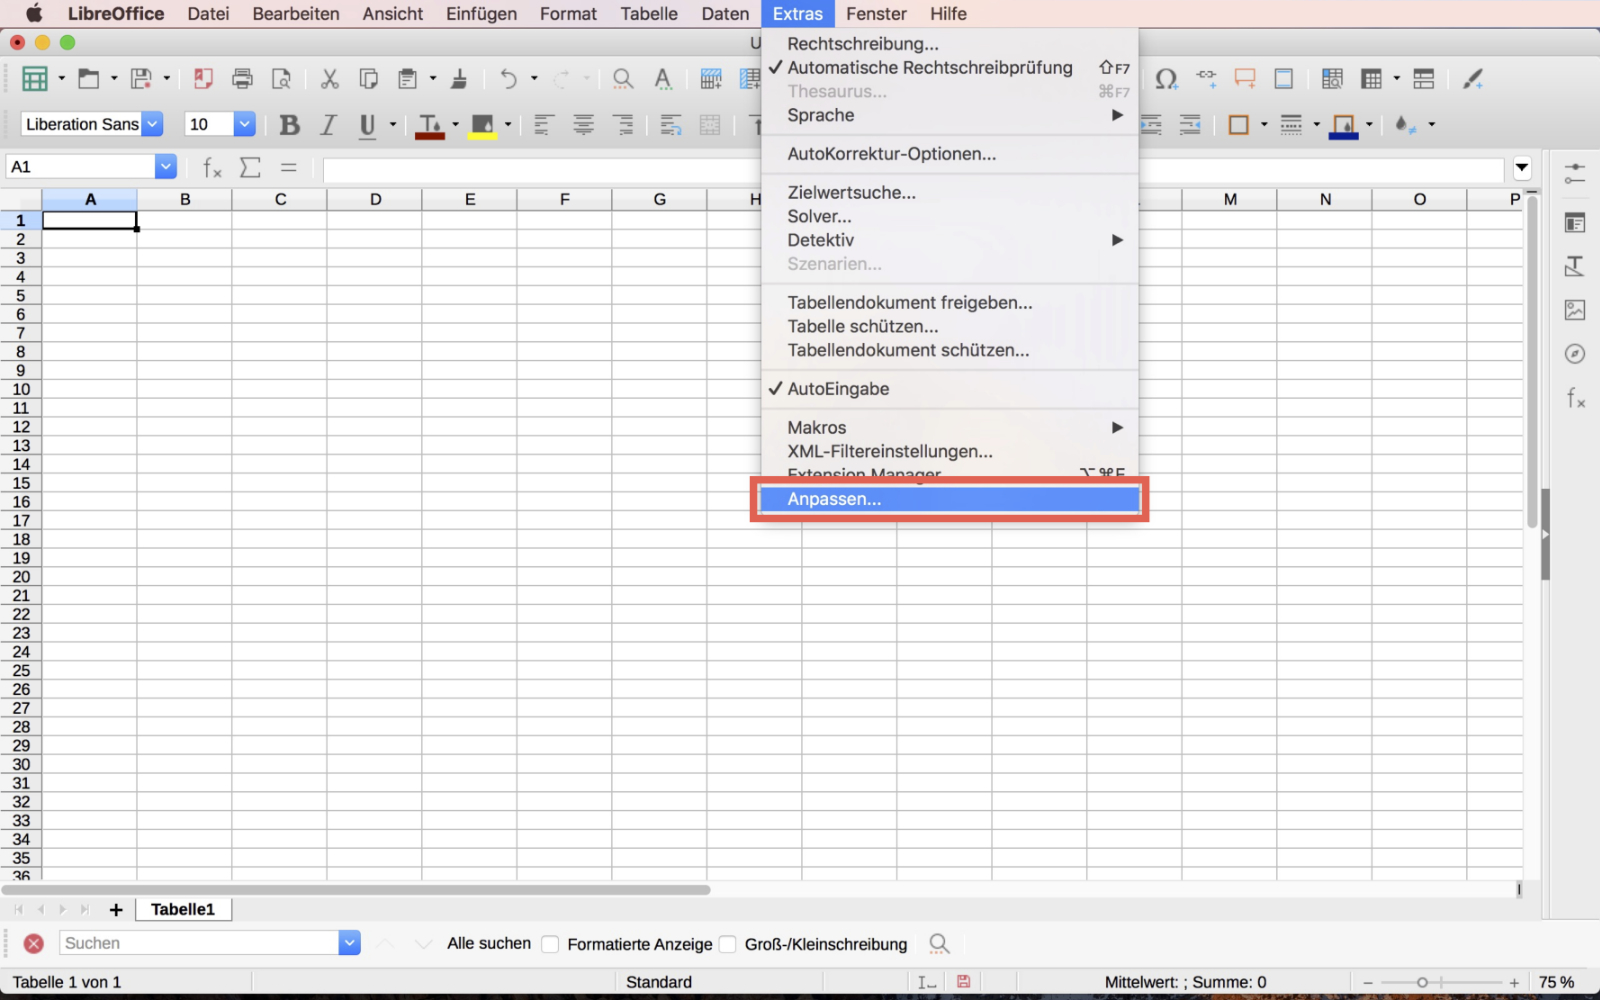
\includegraphics[width=0.9\textwidth]{img/Bildschirmfoto_mitKasten/2_Tastenkombination/1.jpg}
		\end{figure}
	\end{onlyenv}
	\begin{onlyenv}<2>
		\begin{figure}[htbp]
			\centering
			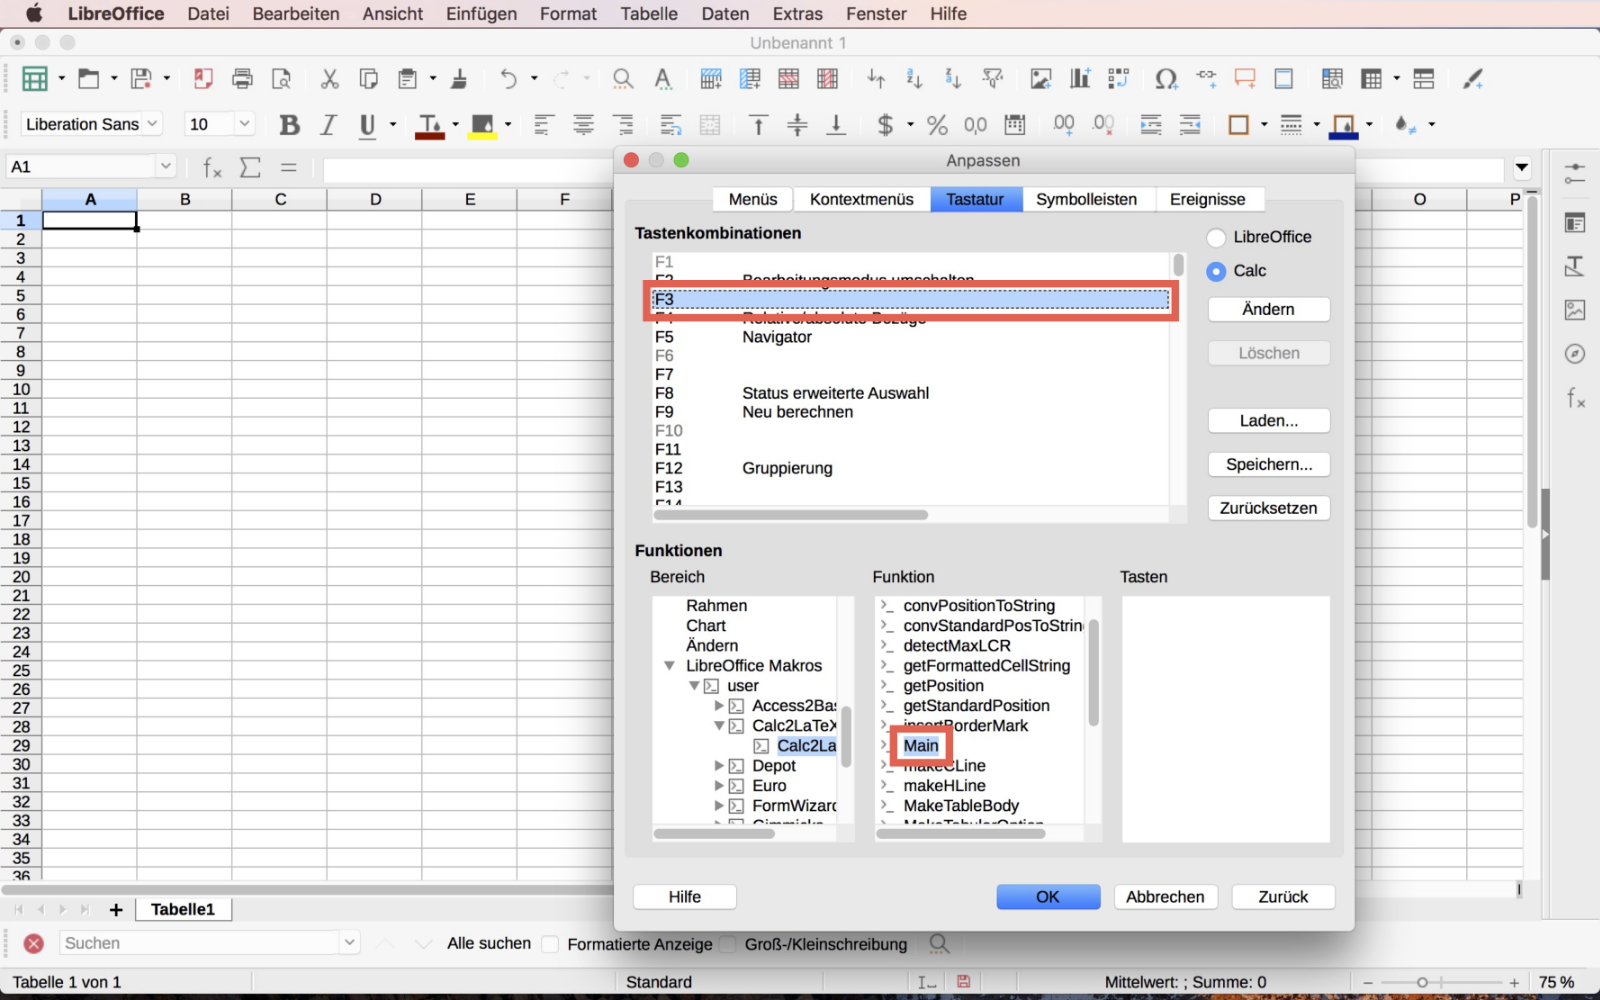
\includegraphics[width=0.9\textwidth]{img/Bildschirmfoto_mitKasten/2_Tastenkombination/2.jpg}
		\end{figure}
	\end{onlyenv}
	\begin{onlyenv}<3>
		\begin{figure}[htbp]
			\centering
			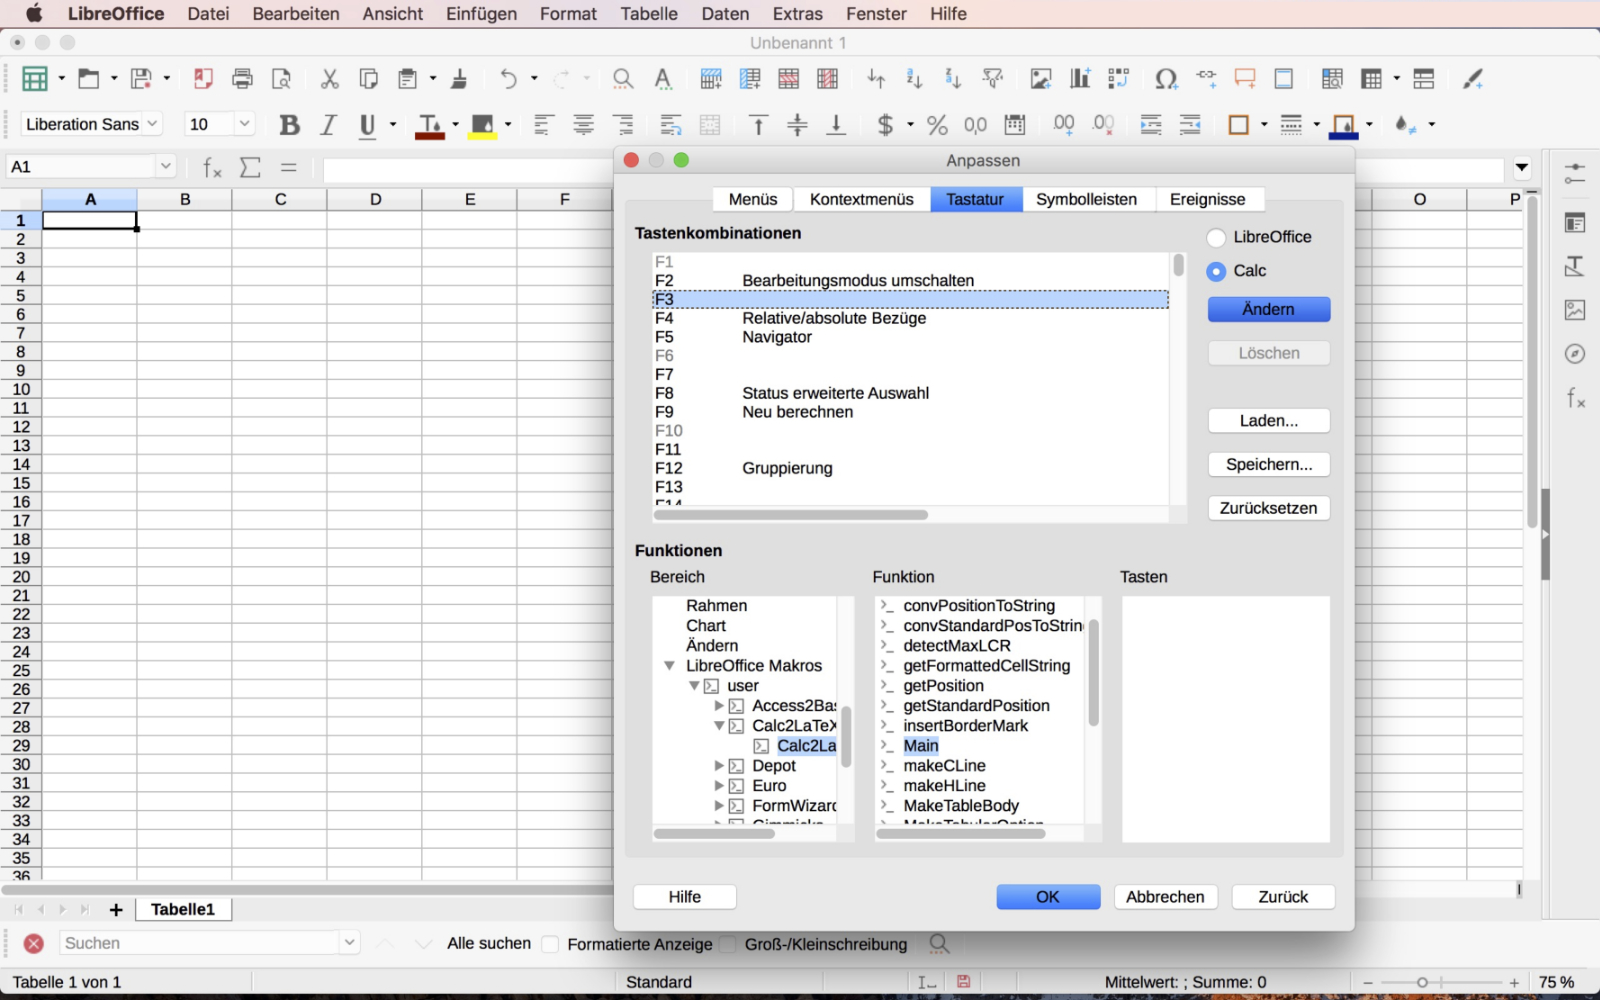
\includegraphics[width=0.9\textwidth]{img/Bildschirmfoto_mitKasten/2_Tastenkombination/3.jpg}
		\end{figure}
	\end{onlyenv}
	\begin{onlyenv}<4>
		\begin{figure}[htbp]
			\centering
			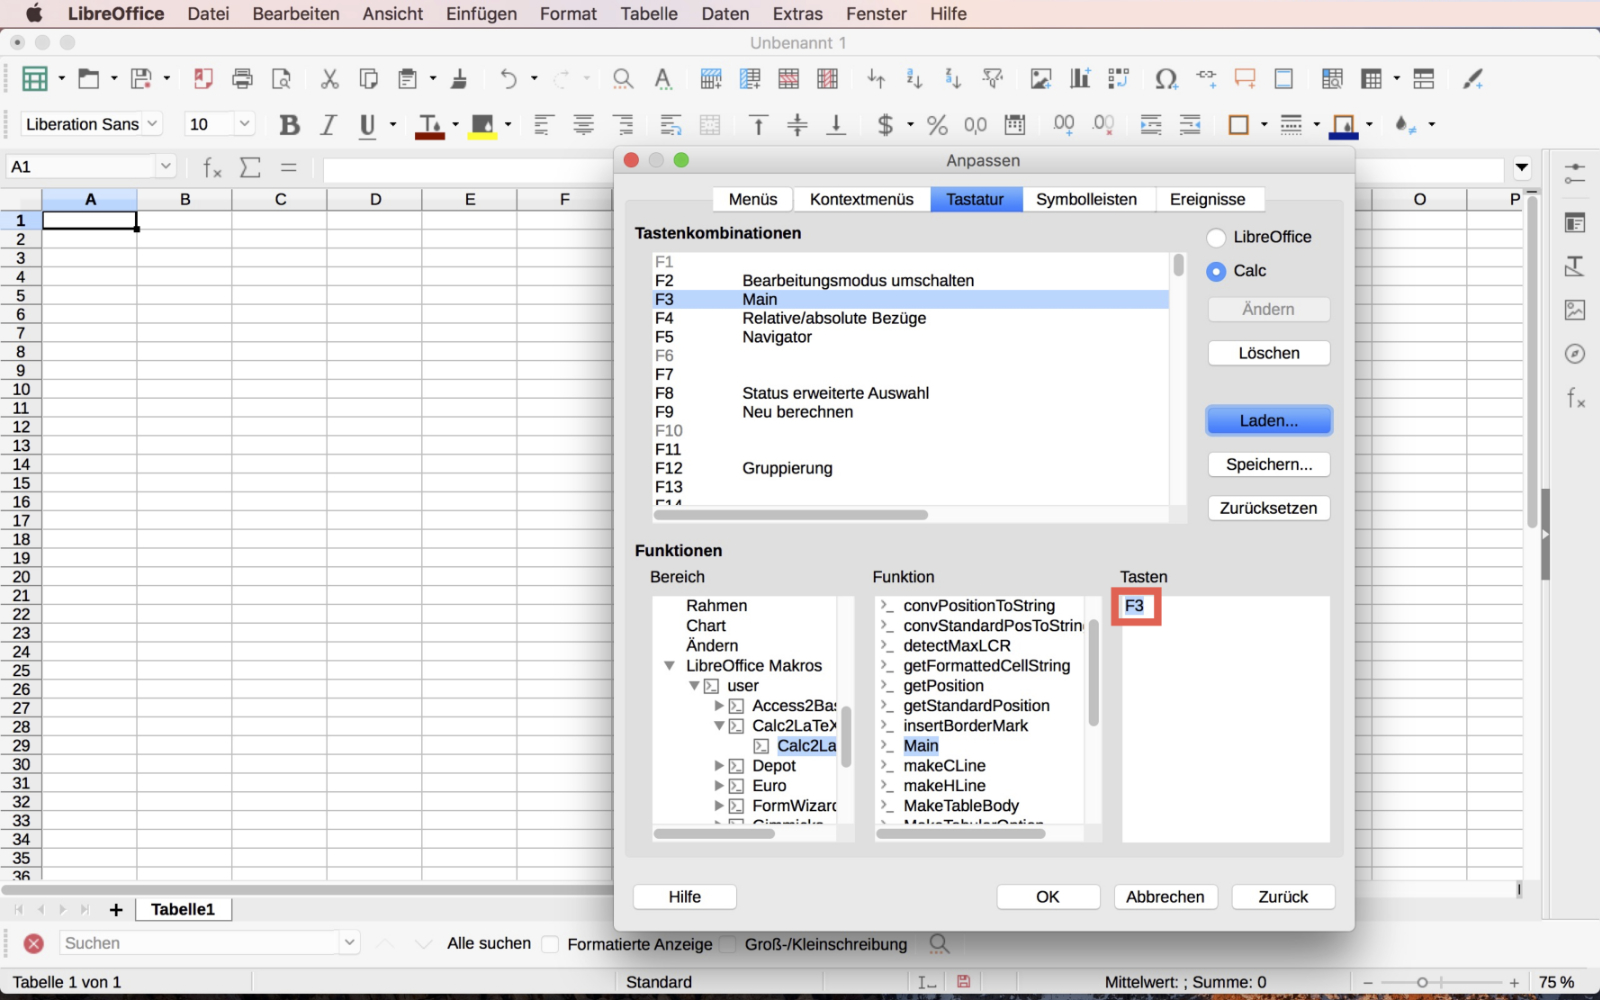
\includegraphics[width=0.9\textwidth]{img/Bildschirmfoto_mitKasten/2_Tastenkombination/4.jpg}
		\end{figure}
	\end{onlyenv}
\end{frame}
%%-----------------------------------------------------------------------------------%
%%---------------------------------------FRAME---------------------------------------%
%%-----------------------------------------------------------------------------------%
\begin{frame}[c]{Erstellen der Tabelle}
	\begin{onlyenv}<1>
		\begin{figure}[htbp]
			\centering
			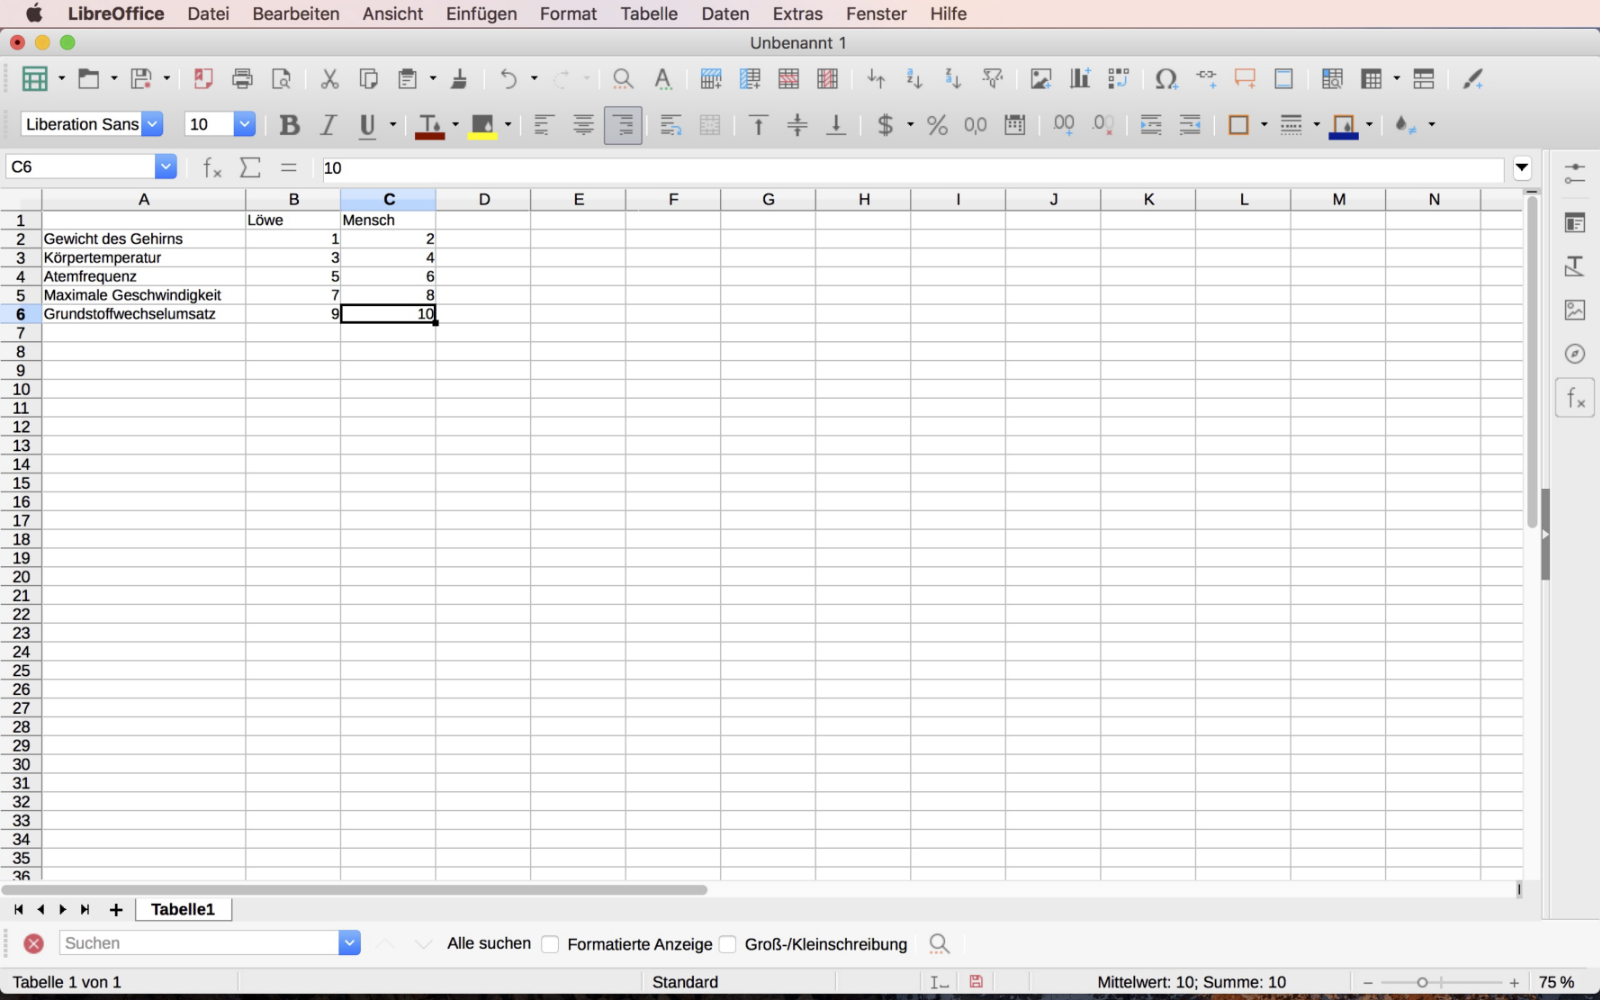
\includegraphics[width=0.9\textwidth]{img/Bildschirmfoto_mitKasten/3_Tabelle/1.jpg}
		\end{figure}
	\end{onlyenv}
	\begin{onlyenv}<2>
		\begin{figure}[htbp]
			\centering
			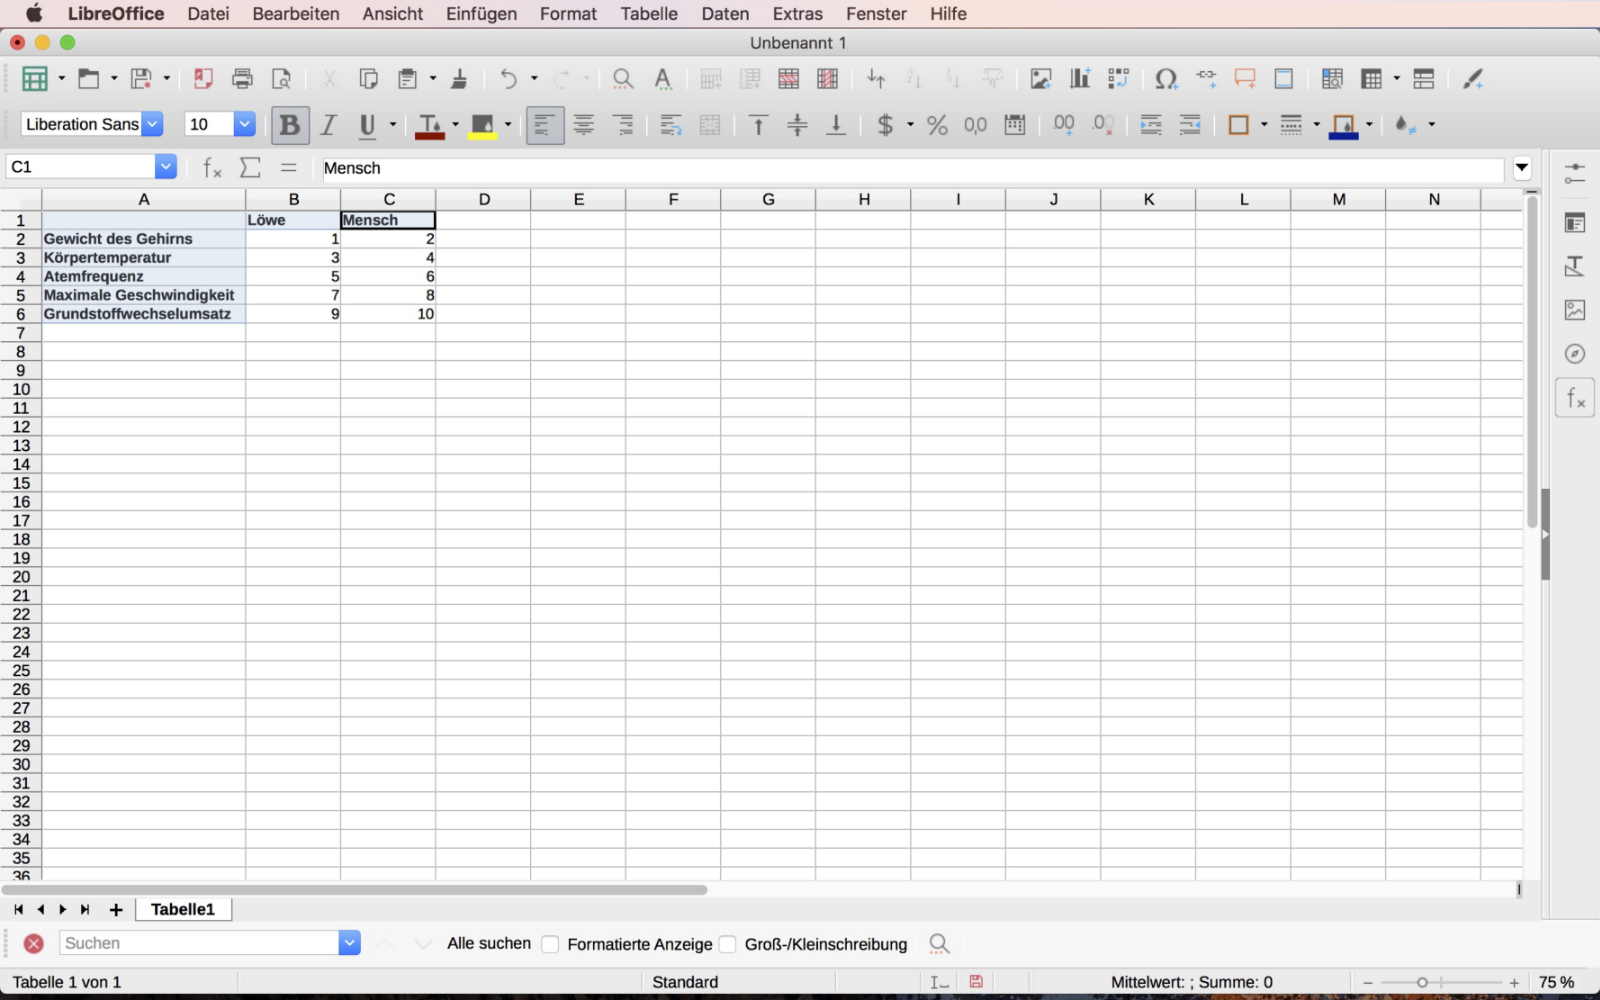
\includegraphics[width=0.9\textwidth]{img/Bildschirmfoto_mitKasten/3_Tabelle/2.jpg}
		\end{figure}
	\end{onlyenv}
	\begin{onlyenv}<3>
		\begin{figure}[htbp]
			\centering
			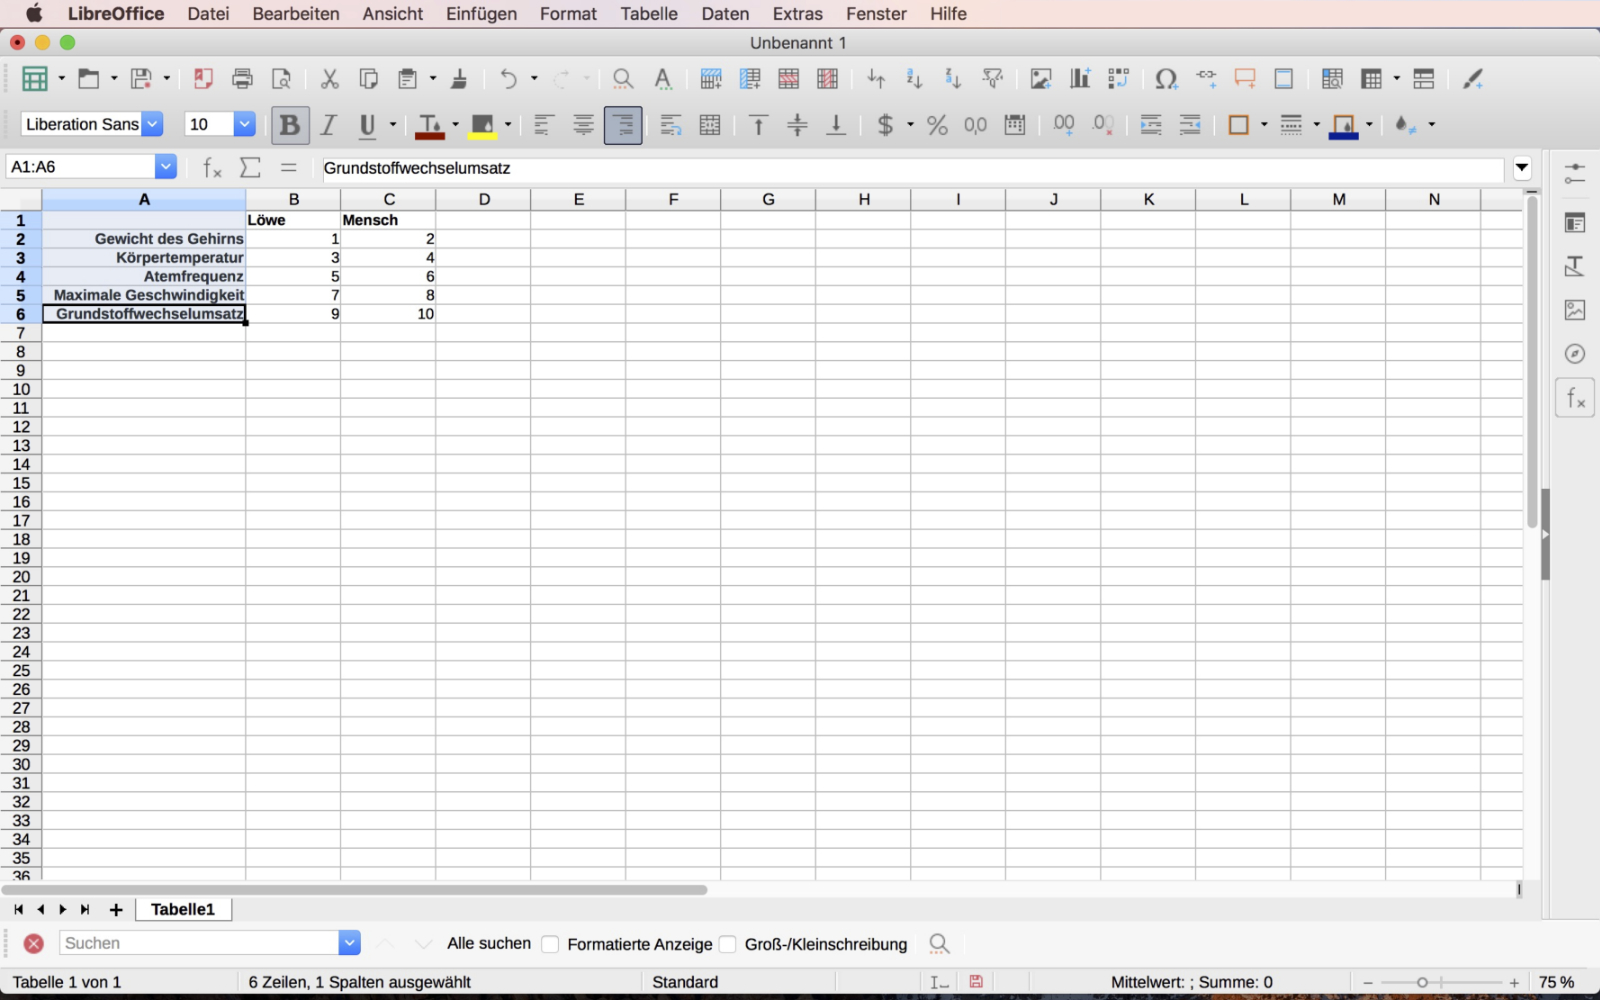
\includegraphics[width=0.9\textwidth]{img/Bildschirmfoto_mitKasten/3_Tabelle/3.jpg}
		\end{figure}
	\end{onlyenv}
	\begin{onlyenv}<4>
		\begin{figure}[htbp]
			\centering
			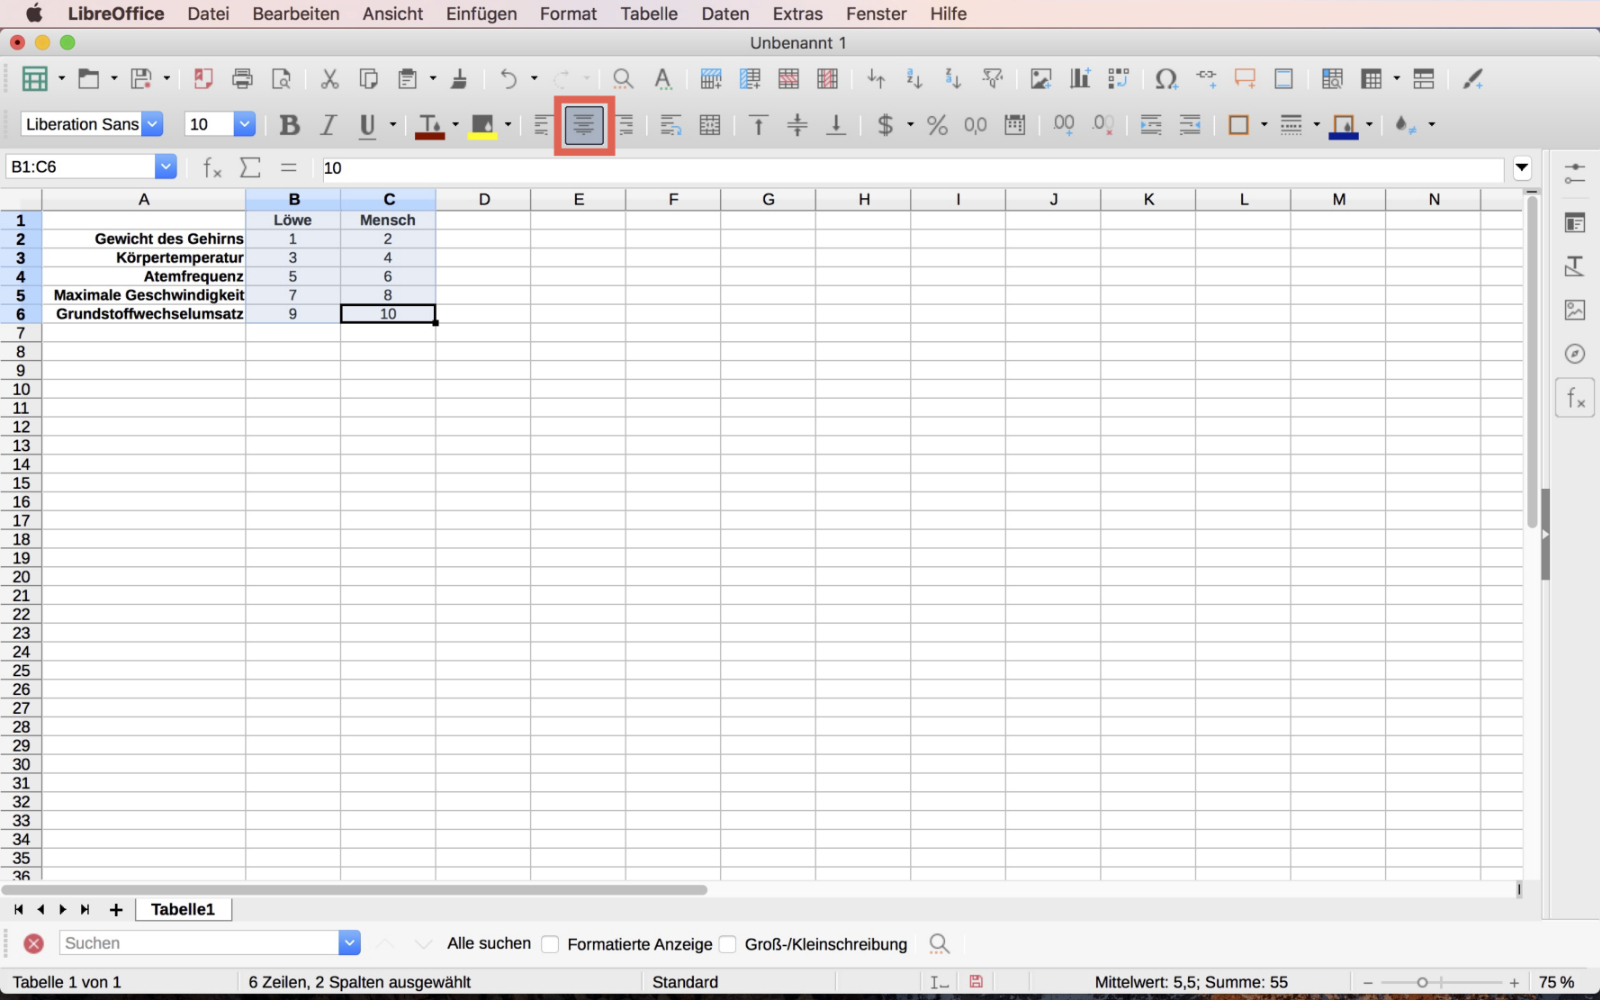
\includegraphics[width=0.9\textwidth]{img/Bildschirmfoto_mitKasten/3_Tabelle/4.jpg}
		\end{figure}
	\end{onlyenv}
	\begin{onlyenv}<5>
		\begin{figure}[htbp]
			\centering
			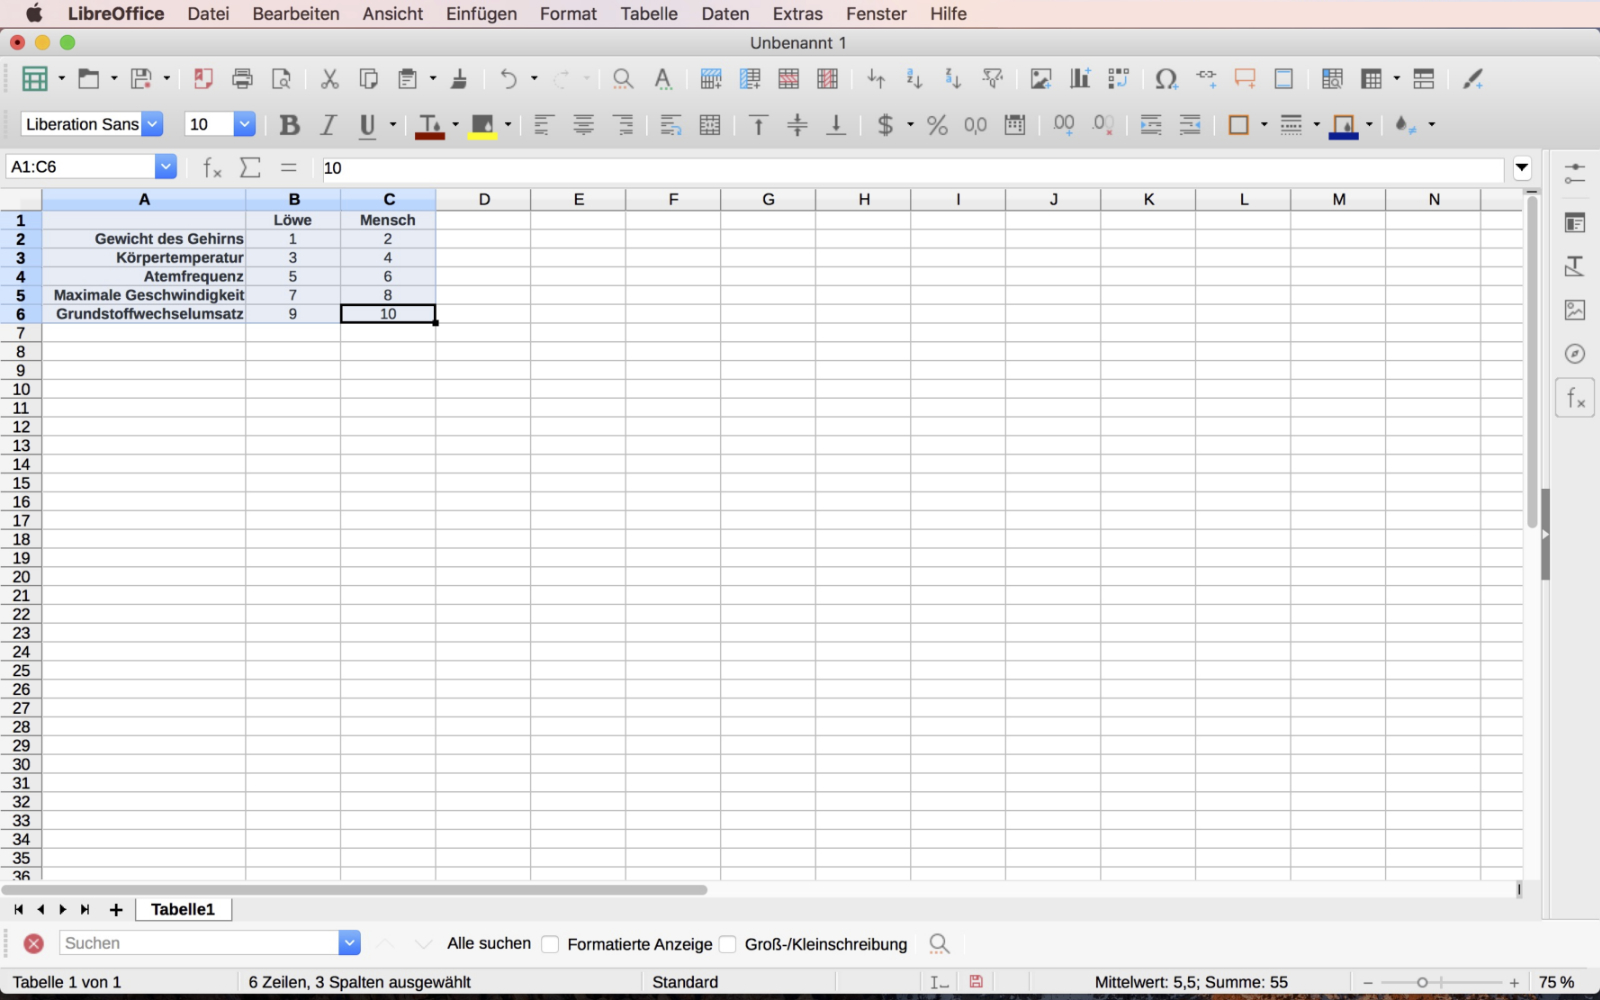
\includegraphics[width=0.9\textwidth]{img/Bildschirmfoto_mitKasten/3_Tabelle/5.jpg}
		\end{figure}
	\end{onlyenv}
\end{frame}
%-----------------------------------------------------------------------------------%
%---------------------------------------FRAME---------------------------------------%
%-----------------------------------------------------------------------------------%
\begin{frame}[c]{Ausführen des Makros}
	\begin{onlyenv}<1>
		\begin{figure}[htbp]
			\centering
			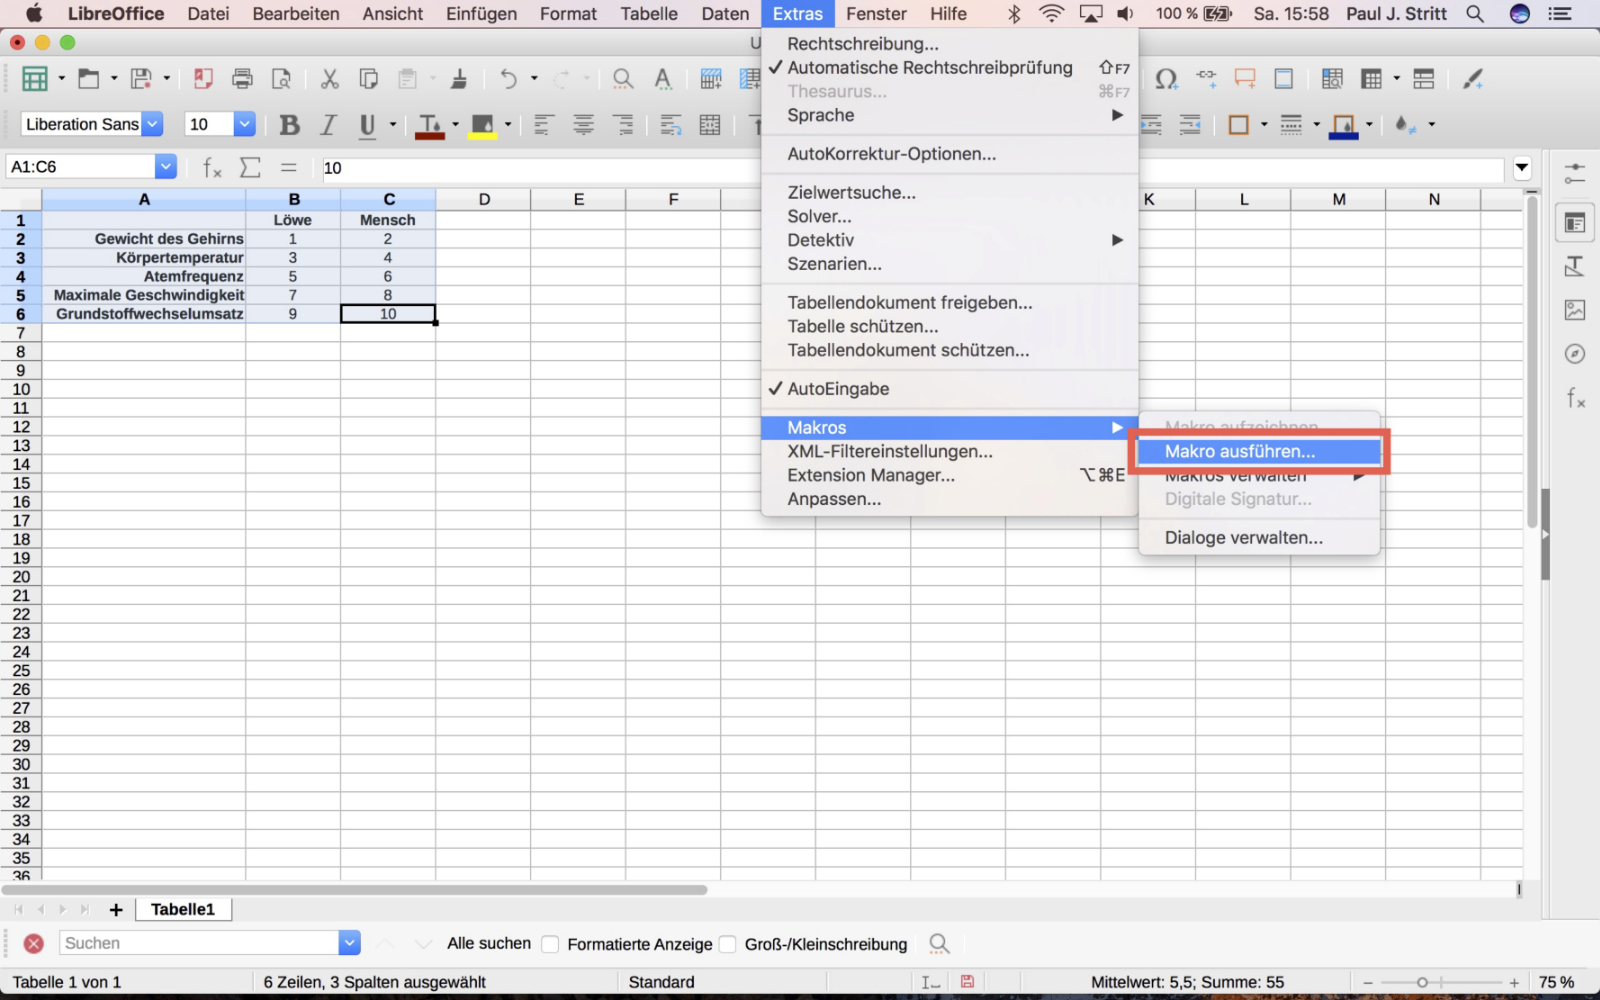
\includegraphics[width=0.9\textwidth]{img/Bildschirmfoto_mitKasten/4_Ausfuhren_Macro/1.jpg}
		\end{figure}
	\end{onlyenv}
	\begin{onlyenv}<2>
		\begin{figure}[htbp]
			\centering
			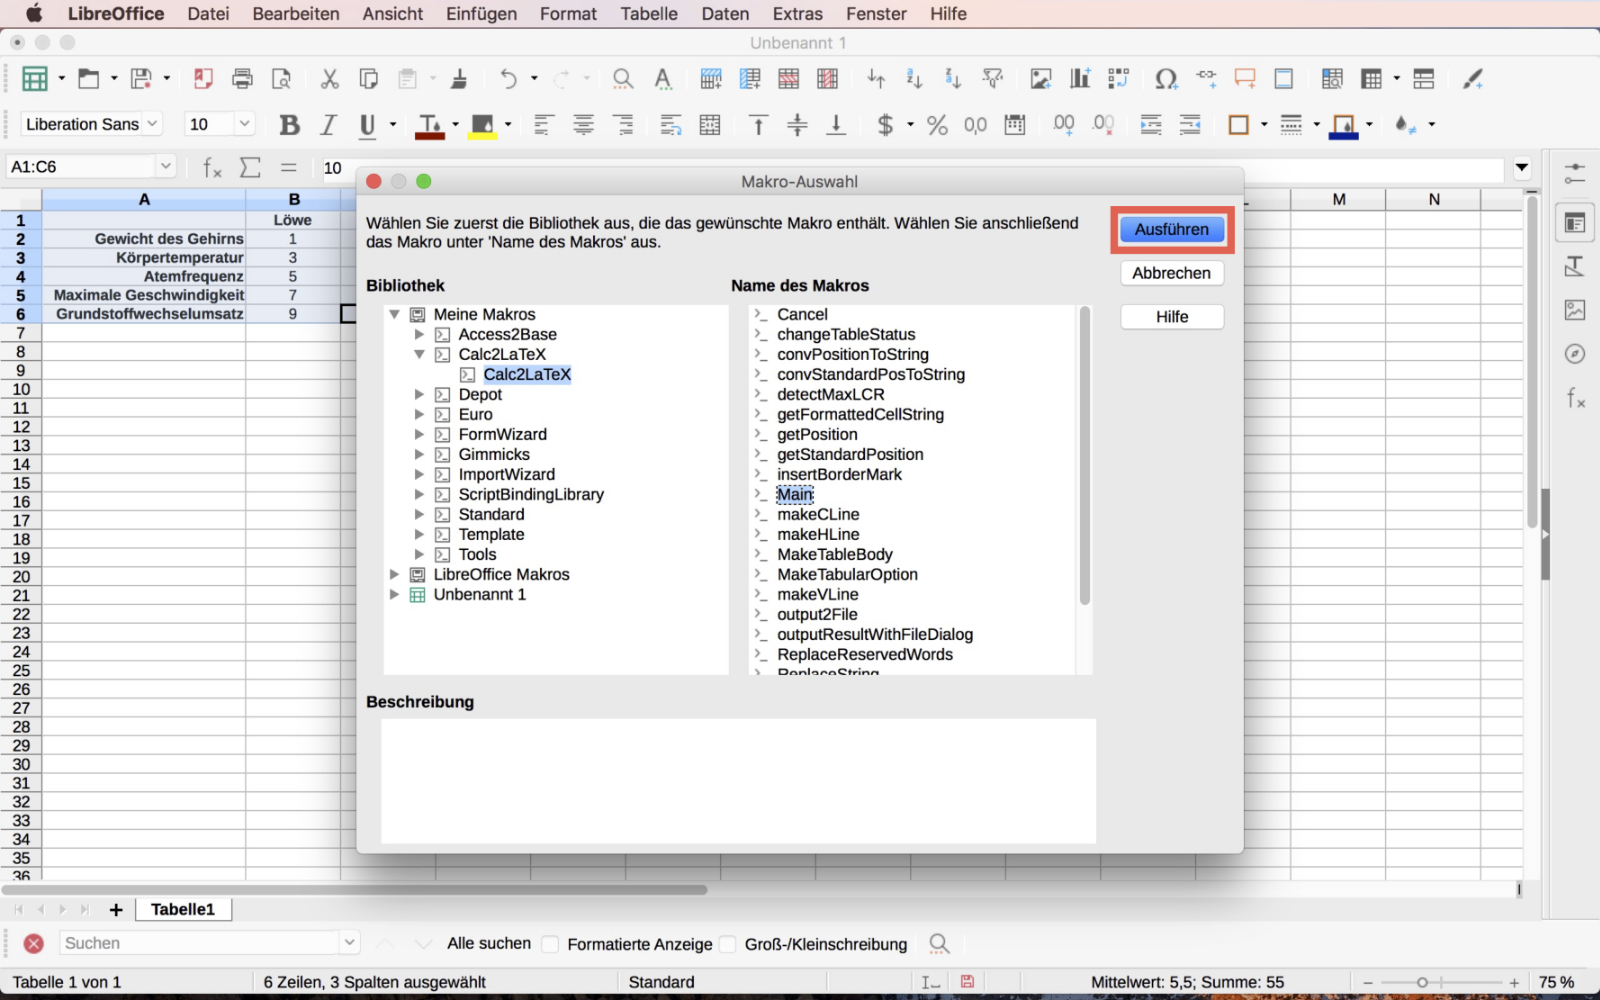
\includegraphics[width=0.9\textwidth]{img/Bildschirmfoto_mitKasten/4_Ausfuhren_Macro/2.jpg}
		\end{figure}
	\end{onlyenv}
	\begin{onlyenv}<3>
		\begin{figure}[htbp]
			\centering
			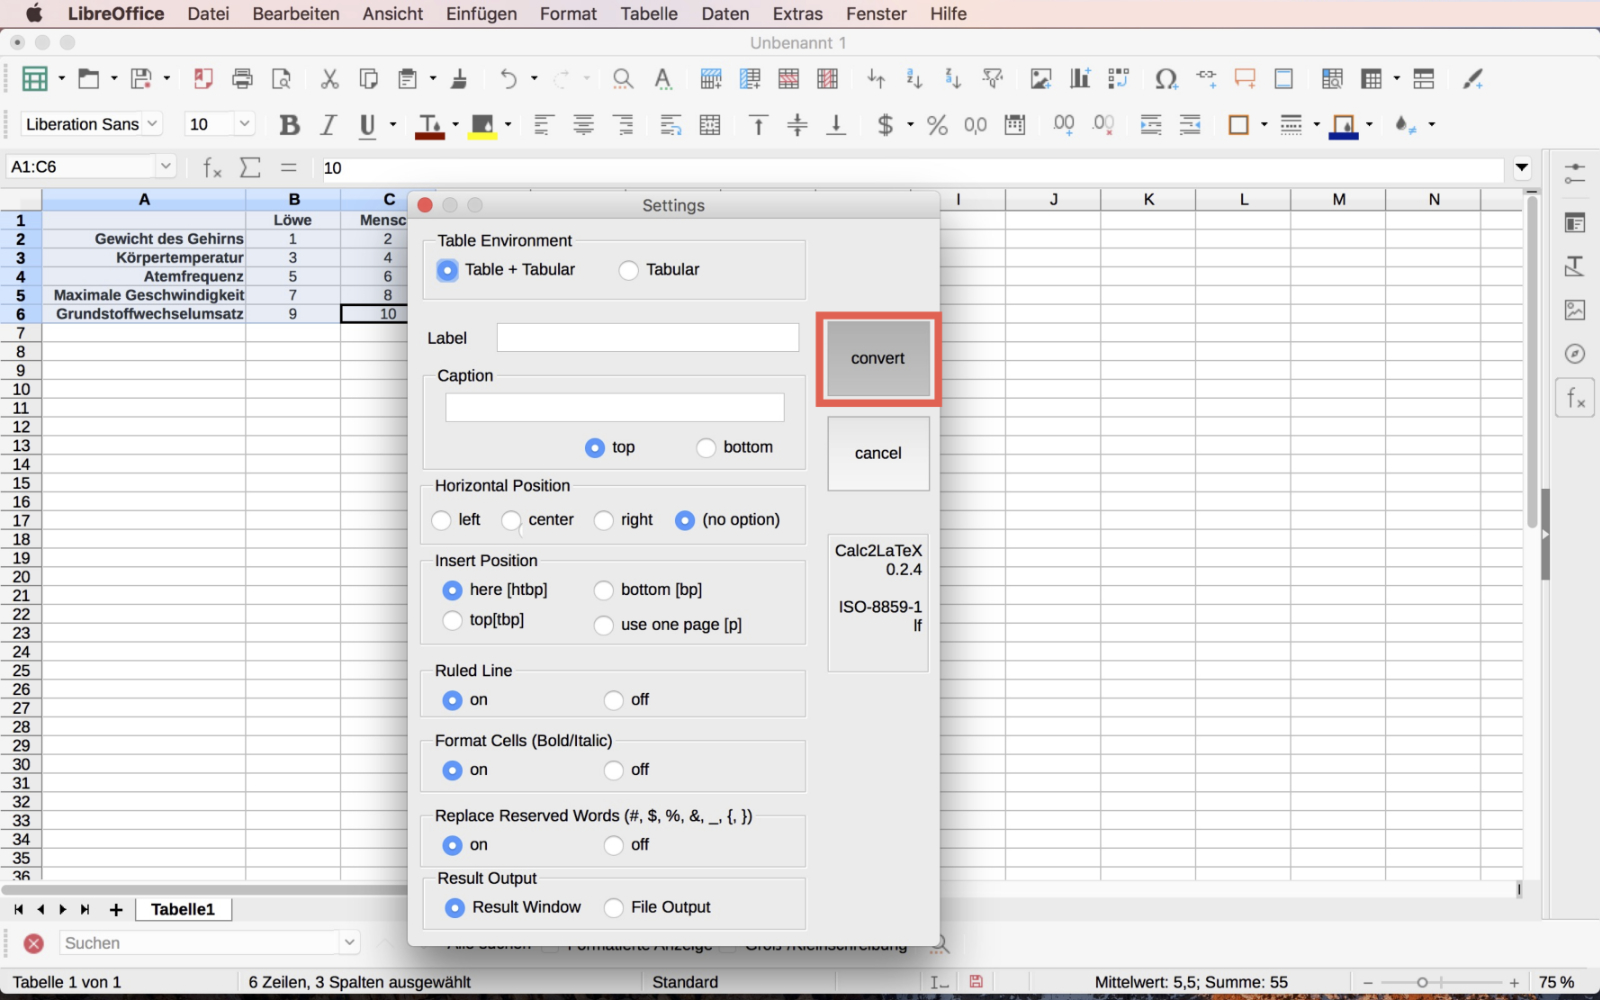
\includegraphics[width=0.9\textwidth]{img/Bildschirmfoto_mitKasten/3_Tabelle/6.jpg}
		\end{figure}
	\end{onlyenv}
	\begin{onlyenv}<4>
		\begin{figure}[htbp]
			\centering
			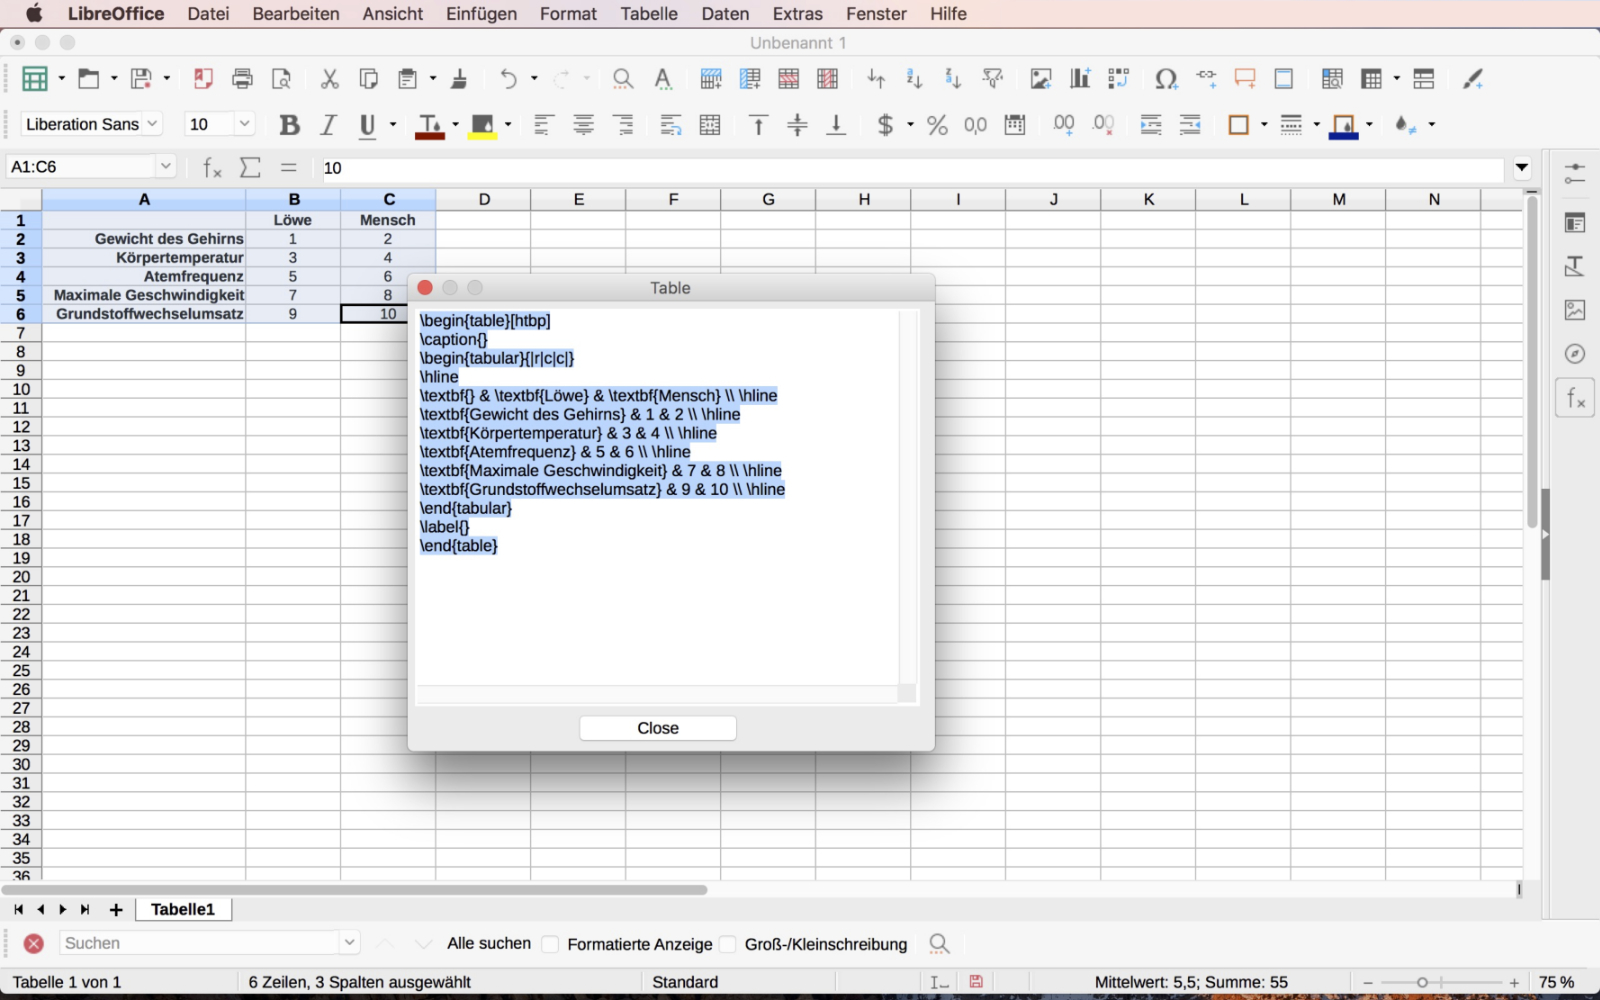
\includegraphics[width=0.9\textwidth]{img/Bildschirmfoto_mitKasten/3_Tabelle/7.jpg}
		\end{figure}
	\end{onlyenv}
\end{frame}
%%-----------------------------------------------------------------------------------%
%%---------------------------------------FRAME---------------------------------------%
%%-----------------------------------------------------------------------------------%
\begin{frame}[fragile]
	\vspace{-0.3cm}
	\begin{Aufgabe}
		\vspace{-0.1cm}
		Füge die erstellte Tabelle als Inhalt von einer neuen, ersten \lstinline[basicstyle=\normalfont\ttfamily\normalsize]|\section| \textrm{\qquote{Vergleich der Körpereigenschaften}} ein.
	\end{Aufgabe}
	\begin{outputbox}
		{\LARGE \textbf{1 Vergleich der Körpereigenschaften}}
		\vspace{-0.3cm}
		\begin{center}
\begin{table}[htbp] 
	\caption{}
	\centering
	\begin{tabular}{|r|c|c|}
		\hline 
		\textbf{} & \textbf{Löwe} & \textbf{Mensch} \\ \hline 
		\textbf{Gewicht des Gehirns} & 1 & 2 \\ \hline 
		\textbf{Körpertemperatur} & 3 & 4 \\ \hline 
		\textbf{Atemfrequenz} & 5 & 6 \\ \hline 
		\textbf{Maximale Geschwindigkeit} & 7 & 8 \\ \hline 
		\textbf{Grundstoffwechselumsatz} & 9 & 10 \\ \hline
	\end{tabular} 
	\label{}
\end{table}
		\end{center}
		\vspace{-0.4cm}
	\end{outputbox}

%	\btVFill\Befehle
%	\begin{center}
%		\begin{tabular}{ll}
%			\toprule
%			\LaTeX\ Befehl								&	Funktion								\\ \midrule
%			\lstinline|\begin{table}...\end{table}|		&	Umgebung für Tabellen					\\
%			\lstinline|\begin{tabular}...\end{tabular}|	&	Erstellt eine Tabelle					\\ 
%			\lstinline|&|								&	Sprung zur nächsten Zelle				\\
%			\lstinline|\\|								&	Neue Zeile								\\
%			\bottomrule
%		\end{tabular}
%	\end{center}
%	\vspace{0.1cm}
\end{frame}
%%-----------------------------------------------------------------------------------%
%%---------------------------------------FRAME---------------------------------------%
%%-----------------------------------------------------------------------------------%
\begin{frame}[fragile]
	\begin{outputbox}
		\vspace{-0.8cm}
		\begin{center}
\begin{table}[htbp] 
	\caption{}
	\centering
\begin{tabular}{|r|c|c|}
	\hline 
	\textbf{} & \textbf{Löwe} & \textbf{Mensch} \\ \hline 
	\textbf{Gewicht des Gehirns} & 1 & 2 \\ \hline 
	\textbf{Körpertemperatur} & 3 & 4 \\ \hline 
	\textbf{Atemfrequenz} & 5 & 6 \\ \hline 
	\textbf{Maximale Geschwindigkeit} & 7 & 8 \\ \hline 
	\textbf{Grundstoffwechselumsatz} & 9 & 10 \\ \hline
\end{tabular} 
\label{}
\end{table}

		\end{center}
		
	\end{outputbox}
	\vspace{-0.4cm}
	\begin{lstlisting}
\begin{table}[htbp]
\caption{}
\centering
\begin{tabular}{|r|c|c|}
\hline 
\textbf{} & \textbf{Löwe} & \textbf{Mensch} \\ \hline 
\textbf{Gewicht des Gehirns} & 1 & 2 \\ \hline 
\textbf{Körpertemperatur} & 3 & 4 \\ \hline 
\textbf{Atemfrequenz} & 5 & 6 \\ \hline 
\textbf{Maximale Geschwindigkeit} & 7 & 8 \\ \hline 
\textbf{Grundstoffwechselumsatz} & 9 & 10 \\ \hline
\end{tabular} 
\label{}
\end{table}
	\end{lstlisting}
\end{frame}
%%-----------------------------------------------------------------------------------%
%%---------------------------------------FRAME---------------------------------------%
%%-----------------------------------------------------------------------------------%
\begin{frame}[fragile]
		\begin{outputbox}
			\vspace{-0.8cm}
		\begin{center}
			\begin{tabular}{|r|c|c|}
				\hline
				&	\textbf{Löwe}				& \textbf{Mensch} 	\\ 	\hline
				\textbf{Gewicht des Gehirns}		&			1					& 		2			\\ 	\hline
				\textbf{Körpertemperatur}			&			3					& 		4			\\	\hline
				\textbf{Atemfrequenz}				&			5					& 		6			\\	\hline
				\textbf{Maximale Geschwindigkeit}	&			7					& 		8			\\ 	\hline
				\textbf{Grundstoffwechselumsatz}	&			9					& 		10			\\	\hline
			\end{tabular}
		\end{center}
	
	\end{outputbox}
	\vspace{-0.4cm}
	\begin{lstlisting}
\begin{tabular}{
|				r				|		c		|		c		  |}
\hline
\textbf{}						& \textbf{Löwe}	& \textbf{Mensch} \\ 
\hline
\textbf{Gewicht des Gehirns}	&		1		& 		2	      \\ 
\hline
\textbf{Körpertemperatur}		&		3		& 		4		  \\ 
\hline
\textbf{Atemfrequenz}			&		5		& 		6	      \\ 
\hline
\textbf{Max. Geschwindigkeit}	&		7		& 		8		  \\ 
\hline
\textbf{Grundstoffwechselumsatz}&		9		& 		10	      \\ 
\hline
\end{tabular}
\end{lstlisting}
\end{frame}

%%-----------------------------------------------------------------------------------%
%%---------------------------------------FRAME---------------------------------------%
%%-----------------------------------------------------------------------------------%
\begin{frame}[fragile]
	\begin{Aufgabe}
		Füge die folgenden Trennstriche in die Tabelle ein und gib der Tabelle ein \textbf{Über}schrift \textrm{\qquote{Vergleich von Löwe und Mensch.}}.
	\end{Aufgabe}
	\begin{outputbox}
		\vspace{-0.5cm}
		\begin{center}
\begin{table}[htbp]
	\caption{Vergleich von Löwe und Mensch.}
	\centering
	\begin{tabular}{r|cc}
		\hline 
		\textbf{} & \textbf{Löwe} & \textbf{Mensch} \\ \hline  
		\textbf{Gewicht des Gehirns} & 1 & 2 \\  
		\textbf{Körpertemperatur} & 3 & 4 \\  
		\textbf{Atemfrequenz} & 5 & 6 \\ 
		\textbf{Maximale Geschwindigkeit} & 7 & 8 \\  
		\textbf{Grundstoffwechselumsatz} & 9 & 10 \\ \hline
	\end{tabular} 
	\label{}
\end{table}
		\end{center}

		\vspace{-0.2cm}
	\end{outputbox}
	
	\btVFill\Befehle
	\begin{center}
		\begin{tabular}{ll}
			\toprule
			\LaTeX\ Befehl								&	Funktion								\\ \midrule
			\lstinline|\hline|							&	Horizontaler Trennstrich von Zeilen				\\
			\lstinline/{|Spalte|Spalte|}/								&	Vertikaler Trennstrich von Spalten					\\
			\bottomrule
		\end{tabular}
	\end{center}
	\vspace{0.1cm}
\end{frame}
%%-----------------------------------------------------------------------------------%
%%---------------------------------------FRAME---------------------------------------%
%%-----------------------------------------------------------------------------------%
\begin{frame}[fragile]
	\Code
	\begin{lstlisting}
\begin{table}[htbp]
\caption{Vergleich von Löwe und Mensch.}
\centering
\begin{tabular}{r|cc}
\hline 
\textbf{}							& \textbf{Löwe} & \textbf{Mensch} 	\\  
\hline 
\textbf{Gewicht des Gehirns}		& 1 			& 2 				\\  
\textbf{Körpertemperatur}			& 3				& 4 				\\  
\textbf{Atemfrequenz}				& 5				& 6 				\\ 
\textbf{Maximale Geschwindigkeit}	& 7 			& 8 				\\  
\textbf{Grundstoffwechselumsatz}	& 9 			& 10 				\\ 
\hline
\end{tabular} 
\label{}
\end{table}
	\end{lstlisting}
\end{frame}
%%%-----------------------------------------------------------------------------------------------%
%%%------------------------------------------SUBSECTION-------------------------------------------%
%%%-----------------------------------------------------------------------------------------------%
%\subsection{Tabellen- und Abbildungsverzeichnisse}
%\begin{frame}[c]
%	\begin{center}
%		\large Tabellen- und Abbildungsverzeichnisse
%	\end{center}
%\end{frame}
%\note{
%- Vor allem in längeren Dokumenten praktisch\\
%- beim AP vielleicht eher nicht notwendig (?)}
%%-----------------------------------------------------------------------------------%
%%---------------------------------------FRAME---------------------------------------%
%%-----------------------------------------------------------------------------------%
%\begin{frame}[fragile]
%	\begin{center}
%		\begin{tabular}{lp{8cm}}
%			\toprule
%			\LaTeX\ Befehl					&	Funktion								\\ \midrule
%			\lstinline|\listoffigures|		&	Erstellt ein Verzeichnis aller Abbildungen im Dokument\newline(genauer: aller \lstinline[basicstyle=\normalsize\normalfont]|\begin{figure}...\end{figure}| Umgebungen)		\\
%			\lstinline|\listoftables|		&	Selbe Funktionalität, bloß für \lstinline[basicstyle=\normalsize\normalfont]|\begin{table}...\end{table}|			\\
%			\bottomrule
%		\end{tabular}
%	\end{center}
	
%	\pause\btVFill
%	\begin{Aufgabe}
%		Füge am Ende des Dokuments ein Tabellen- und ein Abbildungsverzeichnis ein.
%	\end{Aufgabe}
%	\vspace{0.3cm}
%\note<1>{
%- kann nur die Verzeichnisse erstellen, welche sich in den entsprechenden Umgebungen befinden - das ist der grund für \textrm{begin table ... end table} und \textrm{begin figure ... end figure}}
%\end{frame}
%-----------------------------------------------------------------------------------%
%---------------------------------------FRAME---------------------------------------%
%-----------------------------------------------------------------------------------%
%\begin{frame}[fragile]
%	\Code
%	\begin{lstlisting}
%\listoffigures
%\listoftables
%	\end{lstlisting}
%\end{frame}
\end{document}